\listfiles
\documentclass[12pt]{report}\usepackage[]{graphicx}\usepackage[]{color}
%% maxwidth is the original width if it is less than linewidth
%% otherwise use linewidth (to make sure the graphics do not exceed the margin)
\makeatletter
\def\maxwidth{ %
  \ifdim\Gin@nat@width>\linewidth
    \linewidth
  \else
    \Gin@nat@width
  \fi
}
\makeatother

\usepackage{Sweavel}



\usepackage[intoc]{nomencl}
\textwidth=6in \oddsidemargin=0.5in \topmargin=-0.5in
\textheight=9in  % 9in must include page numbers
\textfloatsep = 0.4in 
\addtocontents{toc}{\vspace{0.4in} \protect \hfill Page\endgraf} 
\addtocontents{lof}{\vspace{0.2in} \hspace{0.13in} \ Figure \protect \hfill Page\endgraf} \addtocontents{lot}{\vspace{0.2in} \hspace{0.13in} \ Table \protect\hfill Page\endgraf}

%%%%%%%%%%%%%%%%%%%%%%%%%%%%%%%
%-------------- USE PACKAGE-----------------------------------------%
%%%%%%%%%%%%%%%%%%%%%%%%%%%%%%%

%\usepackage[natbibapa]{apacite}
\usepackage{array}
\newcolumntype{L}{>{\centering\arraybackslash}m{5cm}}
\newcolumntype{R}{>{\centering\arraybackslash}m{2cm}}

\usepackage{amsmath}
\usepackage{mathtools}
\usepackage{longtable}
\usepackage{graphicx}
\graphicspath{ {/Users/mollyolson/Documents/Vanderbilt/Masters_Thesis/ThesisRepo/} }
\usepackage{multirow}
\usepackage[font=singlespacing]{caption}
%\usepackage{caption}
%\captionsetup{font=scriptsize}
\captionsetup{font=footnotesize}
\usepackage[nottoc,notlof,notlot]{tocbibind}
\renewcommand\bibname{REFERENCES}
%\usepackage[backend=bibtex,style=verbose-trad2]{biblatex}
%\bibliography{/Users/mollyolson/Documents/Vanderbilt/Masters_Thesis/ThesisWork/thesisBib.bib}

%\usepackage{cite}


\usepackage{setspace}
\usepackage{titlesec}
\usepackage{tgschola}
\usepackage{color}
\usepackage[left=1.5in,right=1in,top=1in,bottom=1in]{geometry}
\usepackage[table]{xcolor}
 \usepackage{amsfonts}
 \usepackage{amsmath}
 \usepackage{amsbsy,bm}
 \usepackage{amssymb}
\usepackage{graphicx}
 \usepackage{setspace}
 \usepackage{rotating}
 \usepackage{float}
 \usepackage{stmaryrd}
 \usepackage{multirow}
 \usepackage{color}
 \usepackage{soul}
 \usepackage{caption}
\usepackage{eepic}
\usepackage{colortbl}
%\usepackage[numbers]{natbib}
%\usepackage{natbib}
%\usepackage{natbib}
%\setcitestyle{citesep={;}, aysep={,}}
\newcommand\harvardand{\&}

%\renewcommand{\bibname}{References}




\usepackage{multirow}
\usepackage{setspace}
\usepackage{indentfirst}
\usepackage{titlesec}
\usepackage{subfig}
\usepackage[mathscr]{euscript}
\usepackage[titletoc,title]{appendix}
\usepackage[titletoc]{appendix}
\usepackage[tocgraduated]{tocstyle}

\usepackage{textcomp}
\usepackage{array}
\usepackage{listings}
\usepackage{setspace}
\usepackage{mathptmx}
\usepackage{colortbl}
\usepackage{graphicx}
\usepackage{amssymb, amsmath}
\usepackage{subfig}
\usepackage{epsfig}
\usepackage{times}
\usepackage{float}
\usepackage{rotating}
\usepackage{makeidx}
\usepackage{url}
\usepackage{multirow}
\usepackage{booktabs}
\usepackage[subfigure, titles]{tocloft}
\usepackage[hidelinks]{hyperref}

\usepackage{acronym}
\usepackage{datetime}
\usepackage{algorithm}
\usepackage{algorithmic}
\usepackage{url, hyperref}
%\usepackage{cleveref}
\renewcommand{\nomname}{LIST OF ABBREVIATIONS}
\makenomenclature
\graphicspath{{images/}}
\DeclareGraphicsExtensions{.pdf,.jpeg,.png,.PNG, .eps, .tiff}

\urlstyle{same}

\usepackage{makecell}
\usepackage{titletoc}
\usepackage{appendix}
\usepackage[nottoc]{tocbibind}
\setcounter{secnumdepth}{7}
\setcounter{tocdepth}{7}
\usepackage{lscape}

\DeclarePairedDelimiter\ceil{\lceil}{\rceil}
\DeclarePairedDelimiter\floor{\lfloor}{\rfloor}

%%%%%%%%%%%%%%%%%%%%%%%%%%%%%%%
%-------------- NEW COMMANDS-------------------------------------%
%%%%%%%%%%%%%%%%%%%%%%%%%%%%%%%
%new chapter/section and subsection commands
\newcommand{\hsuchapter}[1]{\chapter*{#1} \addcontentsline{toc}{chapter}{#1} } 
\newcommand{\hsusection}[1]{\section*{#1} \addcontentsline{toc}{section}{#1} } 
\newcommand{\hsusubsection}[1]{\subsection*{#1} \addcontentsline{toc}{subsection}{#1} } 

%%%%%%%Configure Table of Contents%%%%%%%%%%%%
\renewcommand{\contentsname}{TABLE OF CONTENTS}
\renewcommand{\cftchapfont}{\normalfont}
\renewcommand{\cftchappagefont}{\normalfont}
\renewcommand{\cftchapleader}{\cftdotfill{\cftdotsep}}

%%%%%%%Configure List of Figures%%%%%%%%%%%%
\renewcommand{\listfigurename}{LIST OF FIGURES}
\setlength{\cftbeforefigskip}{0.2in}

%%%%%%%Configure List of Tables%%%%%%%%%%%%
\renewcommand{\listtablename}{LIST OF TABLES}
\setlength{\cftbeforetabskip}{0.2in}

%%%%%% Configure ABSTRACT %%%%%%
\usepackage{abstract}
\renewcommand{\abstractname}{ABSTRACT}




%%%%%%%Configure Bibliography%%%%%%%%%%%%
\renewcommand{\bibname}{ \texorpdfstring{{REFERENCES\vspace{10mm}}}{REFERENCES}   }

%%%%%%%%%%%%%%%%%%%%%%%%%%%%%%%
%-------------- CONFIGURE CHAPTER HEADINGS--------------%
%%%%%%%%%%%%%%%%%%%%%%%%%%%%%%%



\makeatletter
\def\@makechapterhead#1{
  {\parindent \z@ %\centering
    \LARGE \fontfamily{qcs}\selectfont
    \ifnum \c@secnumdepth >\m@ne
      \if@mainmatter
        \@chapapp\space \thechapter
        \par\nobreak
        \vskip 20\p@
      \fi
    \fi
    \interlinepenalty\@M
    #1\par\nobreak
    \vskip 40\p@
  }}
\def\@schapter#1{\if@twocolumn
                   \@topnewpage[\@makeschapterhead{#1}]%
                 \else
                   \@makeschapterhead{#1}%
                   \@afterheading
                 \fi}
\def\@makeschapterhead#1{
  {\parindent \z@ \centering
    \large
    \interlinepenalty\@M
    #1\par\nobreak
    \vskip 10\p@
  }}




%%% this configure the linespace in the table of content
%%% code is complicated and ugly but it works
\newlength{\li}\setlength{\li}{14.48pt}
\newlength{\di}\setlength{\di}{-3.5mm}
\def\@chapter[#1]#2{\ifnum \c@secnumdepth >\m@ne
      \refstepcounter{chapter}%
      \typeout{\@chapapp\space\thechapter.}%
      \addcontentsline{toc}{chapter}{\numberline{\thechapter}#1}
         %{\protect\numberline{\thechapter}\uppercase{#1}}%
      \addtocontents{toc}{\protect\vspace{\li}}%
  \else
      %\addcontentsline{toc}{chapter}{\uppercase{#1}}%
      \addcontentsline{toc}{chapter}{#1}
      \addtocontents{toc}{\protect\vspace{\li}}%
  \fi
  \chaptermark{#1}%
  \if@twocolumn
      \@topnewpage[\@makechapterhead{#2}]%
  \else
      \@makechapterhead{#2}%
      \@afterheading
 \fi}


\renewcommand\chapter{\addtocontents{toc}{\protect\addvspace{\li}}%
  \if@openright\cleardoublepage\else\clearpage\fi
  \thispagestyle{plain}%
  \global\@topnum\z@
  \@afterindentfalse
  \secdef\@chapter\@schapter}

%%%%%%%%%%%%%%%%%%%%%%%%%%%%%%%%%%%%%%%%%%%%%%%%%%%%%%%%%%%%%%
%-----------CONFIGURE SECTION HEADINGS------------------%
%%%%%%%%%%%%%%%%%%%%%%%%%%%%%%%%%%%%%%%%%%%%%%%%%%%%%%%%%%%%%%
\renewcommand\section{ \@startsection {section}{1}{\z@}%
                                   {-3.5ex \@plus -1ex \@minus -.2ex}%
                                   {2.3ex \@plus.2ex}%
                                   {\centering\large\fontfamily{qcs}\selectfont}}


                    
%%%%%%%%%%%%%%%%%%%%%%%%%%%%%%%%%%%%%%%%%%%%%%%%%%%%%%%%%%%%%%
%-------------CONFIGURE SUBSECTION HEADINGS- --------%
%%%%%%%%%%%%%%%%%%%%%%%%%%%%%%%%%%%%%%%%%%%%%%%%%%%%%%%%%%%%%%
\renewcommand\subsection{\@startsection {subsection}{2}{\z@}%
                                   {-3.5ex \@plus -1ex \@minus -.2ex}%
                                   {2.3ex \@plus.2ex}%
                                   {\noindent \large \fontfamily{qcs}\selectfont }}
                                  
      
                                   

%%%%%%%Sub-Sub-Section's Not  Supported%%%%%%%%%%%%

%%%%%%%%%%%%%%%%%%%%%%%%%%%%%%%%%%%%%%%%%%%%%%%%%%%%%%%%%%%%%%
%-------CONFIGURE TABLE OF CONTENTS HEADING------%
%%%%%%%%%%%%%%%%%%%%%%%%%%%%%%%%%%%%%%%%%%%%%%%%%%%%%%%%%%%%%%
\renewcommand{\@cftmaketoctitle}{
  \chapter*{\contentsname}
  \addcontentsline{toc}{chapter}{TABLE OF CONTENTS}} 

%%%%%%%%%%%%%%%%%%%%%%%%%%%%%%%%%%%%%%%%%%%%%%%%%%%%%%%%%%%%%%
%------CONFIGURE LIST OF FIGURES HEADING------------%
%%%%%%%%%%%%%%%%%%%%%%%%%%%%%%%%%%%%%%%%%%%%%%%%%%%%%%%%%%%%%%
\renewcommand{\@cftmakeloftitle}{
  \chapter*{\listfigurename}
  Figure \hfill Page
  \addcontentsline{toc}{chapter}{LIST OF FIGURES} } 
  
%%%%%%%%%%%%%%%%%%%%%%%%%%%%%%%%%%%%%%%%%%%%%%%%%%%%%%%%%%%%%%
%--------CONFIGURE LIST OF TABLES HEADING-------------%
%%%%%%%%%%%%%%%%%%%%%%%%%%%%%%%%%%%%%%%%%%%%%%%%%%%%%%%%%%%%%%
\renewcommand{\@cftmakelottitle}{
  \chapter*{\listtablename}
   Table \hfill Page
   \addcontentsline{toc}{chapter}{LIST OF TABLES} }  

\makeatother

\setcounter{section}{-1}     

%%%%%%%%%%%%%%%%%%%%%%%%%%%%%%%%%%%%%%%%%%%%%%%%%%%%%%%%%%%%%%
%---------------------------NEW COMMANDS-------------------------%
%%%%%%%%%%%%%%%%%%%%%%%%%%%%%%%%%%%%%%%%%%%%%%%%%%%%%%%%%%%%%%
\newcommand{\etal}{\emph{et al.}}
\newcommand{\leftsup}[2]{{\vphantom{#2}}^{#1}{#2}}
\newcommand{\leftsub}[2]{{\vphantom{#2}}_{#1}{#2}}
\newcommand{\leftsupsub}[3]{{\vphantom{#3}}^{#1}_{#2}{#3}}

\DeclareMathOperator*{\assembly}{\textbf{\Large A} }

\definecolor{lightblue}{rgb}{.90,.95,1} 
\newcommand{\hllb}[1]{
	\sethlcolor{lightblue}
	\hl{#1}
	\sethlcolor{yellow}
	}

\newcommand{\hlc}[2][yellow]{{\sethlcolor{#1}\hl{#2}} }

%%%%%%%%%%%%%%%%%%%%%%%%%%%%%%%%%%%%%%%%%%%%%%%%%%%%%%%%%%%%%%
%--------------DEFINE FLOATS----------------------------------------%
%%%%%%%%%%%%%%%%%%%%%%%%%%%%%%%%%%%%%%%%%%%%%%%%%%%%%%%%%%%%%%
 \floatstyle{plain}
 \newfloat{Box}{h}{lob}
 \newcommand{\boxedtext}[3]{
 	\begin{Box} \caption{\small{#1}}
	\hspace{1.cm}
	\fbox{\begin{minipage}[c]{0.85\linewidth} 
	
	\small{#2}
       
       \end{minipage}}
       
       \label{#3}
       \end{Box}
  }

 \begin{document}


%\pagestyle{myheadings} \markright{\today}
%%%%%%%%%%%%%%%%%%%%%%%%%%%%%%%%%%%%%%%%%%%%%%%%%%%%%%%%%%%%%%
%-------------- MAKE TITLE CHANGES HERE---------------------%
%%%%%%%%%%%%%%%%%%%%%%%%%%%%%%%%%%%%%%%%%%%%%%%%%%%%%%%%%%%%%%
\pagenumbering{alph}

\begin{titlepage}
\thispagestyle{empty}\enlargethispage{\the\footskip}%
\begin{center}
	{\setstretch{1.66} {Working Title: A Comparison of Approaches for Unplanned Sample Size Changes in Phase II Clinical Trials}\par }%
	\vskip.4in
	By
	\vskip .3in
	{Molly Olson}
	\vskip .3in
	
	\begin{doublespace}
	Thesis\\
		Submitted to the Faculty of the \\
		Graduate School of Vanderbilt University \\
		in partial fulfillment of the requirements \\
		for the degree of \\ [.1in]
	\end{doublespace}
	
	\MakeUppercase{MASTER OF SCIENCE} \\[.1in]
	in \\[.1in]
	{Biostatistics} \\[.25in]
	June 30, 2017 \\[.25in]
	Nashville, Tennessee
	\vskip .5in
%\end{center}
%%%Uncomment for Signatures%%%
%Approved: \hskip 2.9in Date:\\[1.2em]
%\rule{3.5in}{.5pt} \hskip 0.1in \rule{2in}{.5pt} \\[.01in]
%Professor John D. Doe \\[.14in]
%\rule{3.5in}{.5pt} \hskip 0.1in \rule{2in}{.5pt}  \\[.01in]
%Professor John D. Doe \\[.14in]
%\rule{3.5in}{.5pt} \hskip 0.1in \rule{2in}{.5pt} \\[.01in]
%Professor John D. Doe \\[.14in]
%\rule{3.5in}{.5pt} \hskip 0.1in \rule{2in}{.5pt} \\[.01in]
%Professor John D. Doe \\[.14in]
%\\[.14in]
%%%%%%%%%%%%%%
%%%%%%Uncomment  for Approved Names%%%%%%
\begin{doublespace}
Approved:\\
Tatsuki Koyama, Ph.D. \\
Jeffrey Blume, Ph.D. \\
\end{doublespace}
%%%%%%%%%%%%%%%%%%%%%%%%%%%%%%%%%%%%%%%
\end{center}
\end{titlepage}
 
\doublespacing
\pagenumbering{roman} \setcounter{page}{2}

%\chapter*{The dedication page is optional. If you don't use it, please delete it.}
%\addcontentsline{toc}{chapter}{DEDICATION}
%\vspace{7mm}

%%%%%%%%%%%%%%%%%%%%%%%%%%%%%%%%%%%%%%%%%%%%%%%%%%%%%%%%%%%%%%
%--------------ACKNOWLEDGEMENTS----------- -----------------%
%%%%%%%%%%%%%%%%%%%%%%%%%%%%%%%%%%%%%%%%%%%%%%%%%%%%%%%%%%%%%%
\chapter*{ACKNOWLEDGMENTS}
\addcontentsline{toc}{chapter}{ACKNOWLEDGMENTS}
\vspace{7mm}


%%%%%%%%%%%%%%%%%%%%%%%%%%%%%%%%%%%%%%%%%%%%%%%%%%%%%%%%%%%%%%
%-------------- BEGIN TABLE OF CONTENTS---------------------%
%%%%%%%%%%%%%%%%%%%%%%%%%%%%%%%%%%%%%%%%%%%%%%%%%%%%%%%%%%%%%%
\begin{singlespace}
\tableofcontents
\newpage
\addcontentsline{toc}{chapter}{\listtablename}
\end{singlespace}

%%%%%%%%%%%%%%%%%%%%%%%%%%%%%%%%%%%%%%%%%%%%%%%%%%%%%%%%%%%%%%
%--------------BEGIN LIST OF TABLES------------------------------%
%%%%%%%%%%%%%%%%%%%%%%%%%%%%%%%%%%%%%%%%%%%%%%%%%%%%%%%%%%%%%%
\listoftables

%%%%%%%%%%%%%%%%%%%%%%%%%%%%%%%%%%%%%%%%%%%%%%%%%%%%%%%%%%%%%%
%--------------BEGIN LIST OF FIGURES----------------------------%
%%%%%%%%%%%%%%%%%%%%%%%%%%%%%%%%%%%%%%%%%%%%%%%%%%%%%%%%%%%%%%
\newpage
\addcontentsline{toc}{chapter}{\listfigurename}
\listoffigures
\newpage
%%%%%%%%%%%%%%%%%%%%%%%%%%%%%%%%%%%%%%%%%%%%%%%%%%%%%%%%%%%%%%
%-------------- ABSTRACT-----------------------------------------------%
%%%%%%%%%%%%%%%%%%%%%%%%%%%%%%%%%%%%%%%%%%%%%%%%%%%%%%%%%%%%%%
\addcontentsline{toc}{chapter}{ABSTRACT}
\chapter*{ABSTRACT}

\vspace{7mm}
Oncology phase II clinical trials are often used to evaluate the initial effect of a new regimen to determine if there is warrant further study in a phase III clinical trial. Simon's two-stage design is a commonly used design in specifying sample sizes and critical values in phase II oncology clinical trials. It is common, however, for attained sample sizes in these trials to be different than planned. In this thesis, we examine the problems in hypothesis testing for two stage phase II clinical trial designs when attained sample sizes differ from the planned design. We describe methods for redesigning trials when attained sample sizes that differ from planned and introduce a new method for redesigning a two stage clinical trial when the first stage sample sizes deviates from planned. These methods would primarily be used for prespecifying redesigns for the cases when the Simon-like design does not have planned accrual. We find that the Likelihood approach has more desirable characteristics for deviations from the planned design, though if one wishes to remain with a traditional Frequentist approach, Olson and Koyama's method,an adaptation of a method that Chang \textit{et al.} proposed, may also be appropriate.  
\newpage

\normalsize
\doublespacing
\pagenumbering{arabic}
\setcounter{page}{1}
%%%%%%%%%%%%%%%%%%%%%%%%%%%%%%%%%%%%%%%%%%%%%%%%%%%%%%%%%%%%%%%%%%%%%%%%%%%%%%%%%%%%%%%%%%%%%%%%%%%%%%%%%%%%%%%%%%
%%%%%%%%%%%%%%%%%%%%%%%%%%%%%%%%%%%%%%%%%%%%%%%%%%%%%%%%%%%%%%%%%%%%%%%%%%%%%%%%%%%%%%%%%%%%%%%%%%%%%%%%%%%%%%%%%%
%%%%%%%%%%%%%%%%%%%%%%%%%%%%%%%%%%%%%%%%%%%%%%%%%%%%%%%%%%%%%%%%%%%%%%%%%%%%%%%%%%%%%%%%%%%%%%%%%%%%%%%%%%%%%%%%%%
%%%%%%%%%%%%%%%%%%%%%%%%%%%%%%%%%%%%%%%%%%%%%%%%%%%%%%%%%%%%%%%%%%%%%%%%%%%%%%%%%%%%%%%%%%%%%%%%%%%%%%%%%%%%%%%%%%
%% -----------------------------------WRITING STARTS HERE ------------------------------------------------------%%
%%%%%%%%%%%%%%%%%%%%%%%%%%%%%%%%%%%%%%%%%%%%%%%%%%%%%%%%%%%%%%%%%%%%%%%%%%%%%%%%%%%%%%%%%%%%%%%%%%%%%%%%%%%%%%%%%%
%%%%%%%%%%%%%%%%%%%%%%%%%%%%%%%%%%%%%%%%%%%%%%%%%%%%%%%%%%%%%%%%%%%%%%%%%%%%%%%%%%%%%%%%%%%%%%%%%%%%%%%%%%%%%%%%%%
%%%%%%%%%%%%%%%%%%%%%%%%%%%%%%%%%%%%%%%%%%%%%%%%%%%%%%%%%%%%%%%%%%%%%%%%%%%%%%%%%%%%%%%%%%%%%%%%%%%%%%%%%%%%%%%%%%
%%%%%%%%%%%%%%%%%%%%%%%%%%%%%%%%%%%%%%%%%%%%%%%%%%%%%%%%%%%%%%%%%%%%%%%%%%%%%%%%%%%%%%%%%%%%%%%%%%%%%%%%%%%%%%%%%%


%---------------------------------------------------------------------------------------------------------------%
%------------------------------------------------CHAPTER1------------------------------------------------%
%---------------------------------------------------------------------------------------------------------------%

%% comparison by itself is interesting
%% chang et al design is a little bit better - it is a new contribution so it won't feel like it is only reviews. 
%% make sure that comes out in the paper
%% maybe change the section title

%%%%%%%%%%%%%%%%%%%%%%%%%%%%%%%%%%%%%%%%%%%%%%%%%%%%%%%%%%%%%%
%------------Introduction------------------------------------%
%%%%%%%%%%%%%%%%%%%%%%%%%%%%%%%%%%%%%%%%%%%%%%%%%%%%%%%%%%%%%%
\cftlocalchange{toc}{450pt}{0cm}
\cftaddtitleline{toc}{chapter}{Chapter}{}
\cftlocalchange{toc}{1.55em}{2.55em}
\chapter{Introduction}
\vspace{-7mm}
Oncology phase II clinical trials are often used to evaluate the initial effect of a new regimen to determine if further study is warranted in a phase III clinical trial \cite{Porcher, Simon, Koyama}. Simon's two-stage design \cite{Simon} is a commonly used design in phase II oncology clinical trials. Koyama and Chen \cite{Koyama} point out that it is common for actual sample sizes of these phase II trials to differ from the planned, pre-specified sample sizes. This happens due to unanticipated accruement speed or drop-out rates, and multi-center trials can be delayed in communication of enrollment and response information causing over enrollment. Currently, when attained sample sizes differ from planned, common practice is to treat the attained sample sizes as planned. Though, when achieved sample sizes differ from planned, testing the attained sample sizes as planned leads to invalid inference and hypothesis testing in these cases is not straightforward \cite{Porcher, Koyama}. Therefore, extensions of two-stage designs for hypothesis testing with unplanned sample size changes is essential. \\
\indent Many traditional Frequentist methods have been proposed to handle unplanned sample sizes in the second stage while using the planned stage I sample size; however, our literature review found that only a few traditional Frequentist methods handle unplanned sample sizes in stage I. Moreover, when focusing on deviations in sample sizes in the second stage, many proposed methods are adjusting inference procedures rather than proposing a redesign. Likelihood based designs, can be used to extend Simon's design, offer a nice solution to this problem because these designs offer flexibility in sample size without inflation of type I error rate. Because calculations of p-values are complicated when attained sample sizes are different from planned \cite{Koyama}, we focus on methods that offer redesigns of a planned two-stage design that will be prespecified along with the planned design.\\
\indent In this paper, we discuss the different methods for Simon's design when the attained stage II sample size is different from planned and when attained sample sizes in both stages are different from planned. We review Simon-like designs in chapter 2 and illustrate redesign methods in chapters 3 and 4. In chapter 5, we review a concrete example from a Likelihood-based clinical trial, and in chapter 6, we present results of a numerical and theoretical study comparing traditional Frequentist properties of approaches in the setting where stage I sample size differs from planned are presented.    
%%%%%%%%%%%%%%%%%%%%%%%%%%%%%%%%%%%%%%%%%%%%%%%%%%%%%%%%%%%%%%
%-------------Background-------------------------------------%
%%%%%%%%%%%%%%%%%%%%%%%%%%%%%%%%%%%%%%%%%%%%%%%%%%%%%%%%%%%%%%
\chapter{Background}
\vspace{-7mm}

%------------------------------------------------------------%
%----------- Background on Simon's design -------------------%
%------------------------------------------------------------%
\indent Two-stage designs for clinical trials are common designs for phase II oncology clinical trials \cite{Simon}. In two-stage designs, the null hypothesis $\mbox{H}_0: p \leq p_0$ is tested against the alternative $\mbox{H}_1: p > p_1$, where $p$ is the true response probability, $p_0$ is the highest probability of response that would indicate that the research regimen is uninteresting and $p_1$ is the lowest probability of response that would indicate that the research regimen warrants further investigation. Under these hypotheses, it is required that the type I error rate be less than $\alpha$ and power be greater than $1-\beta$. The general framework of Simon's design includes a sample size and critical value in each of the two stages. Let $n_1$ denote the first stage sample size, $n_t$ the sample size at the end of the second stage, and let $n_t$ be the sample size for the second stage; $n_2 = n_t-n_1$. Let $r_1$ be the first stage critical value, and $r_t$ the critical value for the end of the second stage. Let $X_1$ be the number of successes observed in the first stage and $X_2$ be the number of additional success in the second stage so that $Z_1 \sim \mbox{Binomial}(n_1,p)$ and $X_2 \sim \mbox{Binomial}(n_2,p)$. Also, let $X_t = X_1 + X_2$. In the first stage, $n_1$ subjects are enrolled. If $r_1$ or fewer subjects ($X_1 \leq r_1$) are successes, then the regimen is rejected and the trial is stopped for futility. If $r_1 + 1$ or more subjects are successful, then the trial continues to the second stage by enrolling $n_2$ additional subjects. If $r_t$ or fewer out of the $n_t$ subjects are successful ($X_t = X_1 + X_2 \leq r_t$), the treatment is considered to be futile, otherwise if $X_t \geq r_t + 1$ subjects succeed, the treatment is considered to be effective and will warrant further study.  \\

\indent Let $b$ denote the binomial probability mass function,${n \choose x} p^x(1-p)^{n-x}$ for $x =  1,2,..,n$, and $B$ denote the cumulative binomial distribution function $\sum_{i=0}^x {n \choose i} p^i(1-p)^{n-i}$. The probability of early termination (PET) with a given probability $p$ in two-stage designs is given by PET = $B(r_1, p, n_1) = P_p[X_1 \leq r_1]$. The expected sample size for a given $p$ is then $\mbox{EN} = n_1 + (1-\mbox{PET})n_2$, and the conditional power is then  
\begin{equation}
\begin{aligned}
CP(p) = \sum_{x_2 = r_t-x_1+1}^{n_2} b(x_2, p, n_2)
\end{aligned}
\end{equation}
It then follows that unconditional power, $UCP(p)$, given probability $p$, is given by 

\begin{equation}
\begin{aligned}
1-PR(p) &= 1 - \left( B(r_1, p, n_1) + \sum_{x=r_1+1}^{min[n_1,{r_t}]} b(x, p, n_1) B(r_t-x,p,n_2) \right) \\
&= \sum_{r_1+1}^{n_1} \left\{\sum_{x_2 = r_t-x_1+1}^{n_2} b(x_2, p, n_2) \right\} b(x_1, p, n_1)
\end{aligned}
\end{equation}
and $UCP(p_1) \geq 1-\beta$ and $UCP(p_0) \leq \alpha$ \\


\indent Simon introduced Optimal and Minimax criteria for selecting good designs \cite{Simon}. An Optimal two-stage design is a two-stage design which minimizes the expected sample size under the null hypothesis ($\mbox{EN}_0$). while still satisfying the type I and type II error probability restrictions. The Minimax design will minimize the maximum sample size ($n_t = n_1 + n_2$). Jung \textit{et al.} \cite{Jung} introduced an extension of Simon's designs called Admissible designs that are considered a compromise between Optimal and Minimax. Admissible designs  have similar maximum sample sizes as the Minimax design and a similar $\mbox{EN}_0$ to the optimal design.  These designs minimizes a straight line on the ($n$, $EN$)-plane, $q \times n + (1-q) \times \mbox{EN}$, for some $q \in [0,1]$ \cite{Jung}. Admissible designs satisfy ($\alpha, \beta$) constraints and obtain an expected sample size somewhere between Optimal and Minimax designs. Admissible designs may be attractive because they have agreeable properties of both the Minimax and Optimal design.  Simon's designs do not allow for early termination of the trial for efficacy \cite{Simon}, and we do not consider that design here. We focus this paper two-stage designs that are either Optimal, Minimax, or Admissible. 


%%%%%%%%%%%%%%%%%%%%%%%%%%%%%%%%%%%%%%%%%%%%%%%%%%%%%%%%%%%%%%
%------------------Literature Review-------------------------%
\chapter{Deviation from Planned Sample Sizes In Second Stage}
%%%%%%%%%%%%%%%%%%%%%%%%%%%%%%%%%%%%%%%%%%%%%%%%%%%%%%%%%%%%%%
%%%%%%%%%%%%%%%%%%%%%%%%%%%%%%%%%%%%%%%%%%%%%%%%%%%%%%%%%%%%%%%
%----------Unplanned sample size in the first stage-----------%
%\section{Deviation from Planned Sample Sizes in Second Stage}
%%%%%%%%%%%%%%%%%%%%%%%%%%%%%%%%%%%%%%%%%%%%%%%%%%%%%%%%%%%%%%%%

When over-enrollment occurs in the first stage, a straightforward solution is to perform an interim analysis on the planned number of first stage subjects, and adjust the testing procedure for a sample size in the second stage that may be different than planned. Likewise, it is also straightforward to simply wait for the appropriate enrollment for the first stage when under-enrollment occurs in the first stage. When over- or under-enrollment occurs in the second stage, it is also possible to adjust the testing procedure for the attained enrollment in the second stage.  This is possible under the assumption of non-informative dropouts; stage I is concluded when the number of non-missing subjects is equal to the planned stage I sample size, and if over enrollment occurs in the first stage, those subjects will only be considered for the second stage analysis \cite{Koyama}. Literature exists describing point estimation of the response rate and p-values for hypothesis testing when stage two sample size is modified \cite{Whitehead}\cite{Changpoint}\cite{Guo}\cite{Jungest}\cite{Tsai}\cite{Jungpvalue}\cite{Koyama}. A review of these methods can be found by Porcher \textit{et al}. \cite{Porcher}. Among them is Koyama and Chen who have shown that the p-value in two-stage trials will depend on the design in addition to the attained data and is complicated in the setting of unplanned sample sizes \cite{Koyama}, we only focus on methods that recalculate critical values for hypothesis testing, or redesigns, and will not focus on p-value calculations. Koyama \textit{et al}. propose a method for inference when stage II sample sizes deviate from the planned stage II sample size \cite{Koyama}. Let $n_1, n_t, r_1, r_t, \alpha$ and $\beta$ be the original design parameters as defined earlier. The authors let the first stage remain as planned and propose a redesign of the second stage. The authors first define conditional power, $\mbox{A}(x_1, n_2, p) = P_p[X_2 \geq r_t | X_1 = x_1].$ Using conditional power evaluated at $p_0$, they calculate a new critical value, $r_t^\ast$, by finding the maximum integer, $r_t^\ast$, such that $\mbox{A}^\ast(x_1, n_2^\ast, p_0) \leq \mbox{A}(x_1, n_2, p_0) \equiv P_{p_0}[X_2^\ast \geq r_t^\ast | X_1 = x_1] \leq P_{p_0}[X_2 \geq r_t | X_1 = x_1]$, where $X_2^\ast \sim \mbox{Binomial}(n_2^\ast, p_0)$ and $n_2^\ast$ is the attained stage II sample size. This method will result in a controlled unconditional type I error rate because the new critical value gives a conditional type I error rate that is more conservative than the original conditional type I error rate, regardless of the observed stage II sample size. The authors comment that with the new critical value, $r_t^\ast$, the total number of positive responses required to reject the null hypothesis may be different because it is conditional on the result of the first stage. \\
\indent Zeng \textit{et al.} \cite{Zeng} proposed methodology that attempts to maximize the unconditional power while controlling for the type I error to calculate the stage II critical value for the attained second stage sample size. The authors define $r_2^\ast(x_1)$ to be the new second stage critical value when $x_1 \geq r_1$ and $r_t^\ast \equiv r_2^\ast(x_1) + x_1$. The second stage critical value will be the integer that maximizes 

\begin{equation}
\begin{aligned}
\mbox{Power} = \sum_{x_1 = r_1}^{n_1} {n_1 \choose x_1} p_1^{x_1} (1-p_1)^{n_1 - x_1} \sum_{r_2^\ast(x_1)}^{n_2^\ast} {n_2^\ast \choose x_2} p_1^{x_2} (1-p_1)^{{n_2^\ast}-x_2}
\end{aligned}
\end{equation}

while subject to 
\begin{equation}
\begin{aligned}
 \mbox{Type I error} = \sum_{x_1 = r_1}^{n_1} {n_1 \choose x_1} p_0^{x_1} (1-p_0)^{n_1 - x_1} \sum_{r_2^\ast(x_1)}^{n_2^\ast} {n_2^\ast \choose x_2} p_0^{x_2}(1-p_0)^{{n_2^\ast}-x_2} \leq \alpha
\end{aligned}
\end{equation}
Though it is theoretically possible to find $r_2^\ast$, this problem doesn't have a closed form solution and the computation is exhaustive. Instead, the authors propose a normal approximation for the binomial random variable to ease the computation of power. That is, 
\begin{equation}
\begin{aligned}
\sum_{x_2 = r_2^\ast(x_1)}^{n_2^\ast} {n_2^\ast \choose x_2} p^{x_2} (1-p)^{n_2^\ast - x_2} \approx 1-\Phi \left(\frac{r_2^\ast(x_1) - n_2^\ast p}{\sqrt{n_2^\ast p(1-p)}} \right)
\end{aligned}
\end{equation}

Substituting the above equation in for power and type I error, and using Lagrange multipliers and differentiating with respect to $r_2^\ast$, the problem is then equivalent to solving the equation 
\begin{equation}
\begin{aligned}
\left(\frac{1}{p_0(1-p_0)} - \frac{1}{p_1(1-p_1)} \right) {r_2^\ast}^2 - \frac{2 n_2^\ast (p_0 - p_1)}{(1-p_0)(1-p_1)}r_2^\ast + \frac{{n_2^\ast}^2(p_0-p_1)}{(1-p_0)(1-p_1)}-2n_2^\ast log \left(\frac{\lambda a(x_1)}{b(x_1)}\right)
\end{aligned}
\end{equation}

where $a(x_1) = {n_1 \choose x_1} p_0^{x_1} (1-p_0)^{n_1-x_1}$, $b(x_1) = {n_1 \choose x_1} p_1^{x_1} (1-p_1)^{n_1-x_1}$, and $\lambda$ is the Lagrange multiplier. The new critical value, $r_2^\ast$, is then max$\left(0, min\left(r_2^\ast, n_2^\ast \right) \right)$. The authors suggest searching over a reasonable range of $\lambda$ to find a $\lambda$ such that the type I error is as closed to $\alpha$ as possible. \\

\indent The authors performed a numerical study to compare their method to Koyama and Chen's. They find that, in almost all scenarios that were considered, Zeng \textit{et al.}'s method had more power than Koyama and Chen and this is mostly because Koyama and Chen's method most often results in a lower type I error rate due to controlling of conditional type I error. 



\newpage
%%%%%%%%%%%%%%%%%%%%%%%%%%%%%%%%%%%%%%%%%%%%%%%%%%%%%%%%%%%%%%%%
%---------Unplanned sample sizes in first stage----------------%
\chapter{Deviation from Planned Sample Sizes in First Stage}
%%%%%%%%%%%%%%%%%%%%%%%%%%%%%%%%%%%%%%%%%%%%%%%%%%%%%%%%%%%%%%%%

\indent A straightforward solution to under-enrollment in the first stage is to simply wait until the appropriate enrollment has been reached, hence, why there is little research for this problem. Because accruement of subjects can be unexpected in the first stage, and some situations require early evaluation of the first stage, it is imperative that methods are available to handle situations with attained sample sizes that differ from the planned sample size in stage I. Green and Dahlberg \cite{Green} and Chen and Ng \cite{Chen} propose methods for inference when first stage sample sizes differ from those planned. Recall that $p_0$ is the highest probability of response that would indicate that the research regimen is uninteresting and $p_1$ is the lowest probability of response that would indicate that the research regimen warrants further investigation. The Southwest Oncology Group's standard approach is to use two-stage designs with a type I error rate of 5\% and power of 90\%. Southwest Oncology Group's inference method by suggesting to perform a hypothesis test on $H_0: p=p_1$ versus $H_1: p < p_1$ in the first stage with type I error rate of 2\% and concluding futility if the p-value for this test is $\leq 0.02$. They then suggest testing $H_0: p=p_0$ versus $H_1: p < p_0$ in the second stage at the 0.05 level. The type I error rate of 2\% corresponds to intuition regarding what constitutes evidence in favor of a hypothesis when the sample size is half of the planned total \cite{Green}. Green and Dahlberg extend the SWOG approach by applying this testing method on the attained design, but performing an unadjusted 0.055 level test of $H_0$ based on the attained total sample size at the second stage. The 0.055 level was chosen because of the discreteness of the binomial distribution and to achieve a type I error rate closer to 0.05. The authors demonstrated that this approach controls type I error and achieves desired power only in the limited situation when an overall $\alpha$-level is 0.05, and it is unclear how this method would generalize to any $\alpha$-level \cite{Li}. Li \textit{et al.} also indicates that this limited approach, and particularly testing a hypothesis in the first stage with a type I error rate of 2\%, is arbitrary and lacks theoretical justification. Chang \textit{et al}. \cite{Chang} also point out that Green and Dahlberg's designs can possibly be quite different than the planned design. Chen and Ng \cite{Chen} suggest an approach to unplanned sample sizes by considering a range of sample sizes in both the first and second stages. They search these ranges for the Minimax and Optimal designs that satisfy error constraints using the average probability of termination for all possible first stage sample sizes and average expected sample size for all possible stage I and stage II sample size combinations that they consider \cite{Chen}. Some limitations of this approach are that attained sample sizes may fall outside of the specified ranges, and only the average error probabilities are controlled rather than the actual error probabilities corresponding to the attained sample sizes. Thus, we consider new approaches to unplanned sample sizes in the first stage in both the traditional Frequentist and Likelihood settings. In the interest of prespecifying designs, we focus on deviation from the planned sample size only in the first stage. It is impractical to prespecify limitless combinations of unplanned sample sizes in both the first and second stages.   

%%%%%%%%%%%%%%%%%%%%%%%%%%%%%%%%%%%%%%%%%%%%%%%%%%%%%%%%%%%%%%
%--------------------Chang et al method----------------------%
\section{\textit{Chang et al.} Alternative Designs and Adaptation}
%%%%%%%%%%%%%%%%%%%%%%%%%%%%%%%%%%%%%%%%%%%%%%%%%%%%%%%%%%%%%%
Chang \textit{et al.} \cite{Chang} proposed an alternative design that is an extension of two-stage designs in order to handle unplanned sample sizes in both the first and second stages, though we only consider this extension for over- and under-enrollment in the first stage. This method calculates new critical values for attained sample sizes a priori, and thus one is able to create and pre-specify a new design based on a preferred Simon or Admissible design in defense of the events of unplanned sample sizes. We use this method to pre-specify new designs; that is, we calculate new critical values for different combinations of possible deviations in sample sizes pre-attainment. Because it is desired to stay as closely to the original design as possible for financial and resource planning reasons, we investigate this method while maintaining the original second stage sample size ($n_2$) or original total sample size ($n_t$). Again, let $n_1$, $n_t$, $r_1$, $r_t$, $p_0$, $p_1$, $\alpha$, and $\beta$ be the original, planned design parameters. Now, let $n_1^{\ast \ast}$ be the attained sample size for the first stage and $n_2^{\ast\ast} = n_t - n_1^{\ast\ast}$. Then, the two situations we consider are 1. $n_2^{\ast\ast} = n_t + n_1^{\ast\ast}$ and 2. $n_t^{\ast\ast} = n_1^{\ast\ast} + n_2$. \\
\indent Chang \textit{et al.} proposes a method for updating the stage I critical value based on the following $\beta$-spending function, where m is the attained sample size in the first stage.
\begin{equation}
\begin{aligned}
\beta(m) = \left\{
        \begin{array}{ll}
            \beta_1 m/n_1 & \quad \text{if } m\leq n_1 \\
            \beta_1 + (\beta - \beta_1)(m - n_1)/n_2 & \quad \text{if } m > n_1
        \end{array}
    \right.
\end{aligned}
\end{equation}
Where $\beta_1 = \mbox{P}(X_1 \leq r_1 \vert n_1, p = p_1)$ is the stage I type II error probability.
We then find a new stage one critical value, $s_1$, using this probability spending function such that $P(X_1 \leq s_1 | n_1^{\ast\ast}) \approx \beta(n_1^{\ast\ast})$, where $\approx$ means ``closest to." After $s_1$ is selected, we then search for an integer for the second stage critical value, $s_t$, that satisfies
\begin{equation}
\begin{aligned}
& P(X_1 > s_1, X_t > s_t | n_1^{\ast\ast}, m_2, p_0) \\
= & \sum_{s_1}^{n_1^{\ast\ast}} P(X_2 > s_t - X_1 | X_1 = x_1) P(X_1 > s_1) \\
 \leq & \alpha \\
\end{aligned}
\end{equation}
where $m_2 = n_2$ or $n_2^{\ast\ast}$. 
Chang \textit{et al.}'s design can be used for any $\alpha$-level and is flexible, close to the original design, and preserves the desired traditional Frequentist type I error rate. \\
%Wu \textit{et al} \cite{Wu} also proposed an adjustment to Simon’s design based on attained sample sizes in both the first and second stages. Because Wu's methods don't work very well \textbf{wording}, we won't consider their method for the remainder of this paper. 
We modify Chang \textit{et al.}'s method because we prefer to be conservative when straying from a desired Simon or Admissible design. We modify the design by selecting $s_1$ such that the new design's probability of early termination under the null ($\mbox{PET}_0^{\ast\ast}$) that is closest to the planned probability of early termination under the null, rather than using a type II error probability spending function. This is conservative because when the attained sample size gets further from the planned sample size, the $\mbox{PET}_0^{\ast\ast}$ can get further from the original design's. By selecting the closest integer such that the $\mbox{PET}_0^{\ast\ast}$ is closest to planned, the probability of early termination is greater under large deviations and this method is consistent with Chang \textit{et al.}'s. We select $s_1$ such that 

\begin{equation}
\begin{aligned}
P(X_1 \leq s_1 | n_1^{\ast\ast}, p_0) \approx P(X_1 \leq r_1 | n_1, p_0)
\end{aligned}
\end{equation}

We then select the stage two critical value, $s_t$, in the same fashion as Chang's design. Another option would be to be choose $s_1$ such that the probability of early termination under the null with the redesign is greater than or equal to the original design. In either case, the designs tend to be close when the attained sample size is close to the original, so we consider the case where the probability of early termination is closest to the original. We call this adaptation to Chang \textit{et al.}'s design ``Olson and Koyama's design"  

%------------------------------------------------------------%
%----------- Background on likelihood design ----------------%
%------------------------------------------------------------%
\section{Likelihood Design}
%\vspace{-5mm}

Briefly, Likelihood methods in phase II designs use the likelihood ratio as a measure of evidence \cite{Ayers}. The Law of Likelihood states that ``if the first hypothesis, $H_1$, implies that the probability that a random variable $X$ take the value $x$ is $P_1(X)$, while the second hypothesis, $H_2$, implies that the probability is $P_2(x)$, then the observation $X=x$ is evidence supporting $H_1$ over $H_2$ if and only if $P_1(x) > P_2(x)$, and the likelihood ratio measures the strength of evidence" \cite{Blume2002}. Define $\mbox{L}_n(p) \sim$ Binomial(n,p) to be 
\begin{equation}
\begin{aligned}
\mbox{L}_n(p) &= P(X \vert p, n) \\
&= {n \choose x} p^x (1-p)^{n-x} \\
& \propto p^x (1-p)^{n-x}
\end{aligned}
\end{equation}
Here, the likelihood ratio is 
\begin{equation}
\begin{aligned}
\mbox{LR}_n & = \frac{\mbox{L}_n(p_0)}{\mbox{L}_n(p_1)} \\
&= \frac{p_0^{x_t}(1-p_0)^{n_t-x_t}}{p_1^{x_t}(1-p_1)^{n_t-x_t}} \\
\end{aligned}
\end{equation}
The hypothesis that is better supported is the hypothesis that signs a higher probability to the observed events \cite{Blume2002}. If the likelihood ratio is greater than 1, the evidence favors $H_1$ over $H_2$, and if the likelihood ratio is less than 1, the evidence favors $H_2$ over $H_1$. The likelihood ratio is continuous on the scale of (0,$\infty$) and this scale can be broken up into categories such as `weak' and `strong' evidence \cite{Blume2002}. We make the following decision at the conclusion of the study. If the $\mbox{LR}_n \in [0, 1/k]$, there is evidence for the null hypothesis, if $\mbox{LR}_n \in [1/k,k]$, there is weak evidence for either hypothesis, and if $\mbox{LR}_n \in [k,\infty]$, there is evidence for the alternative hypothesis, where $k$ is a value that is a benchmark for distinguishing strength of evidence. \\

To illustrate the use of the likelihood ratio as a measure of evidence, consider a study that is interested in the response rate of patients. Suppose a researcher is interested in looking at the response (yes/no) of 50 patients, while testing the null hypothesis, $H_0: p = 0.3$, versus $H_1: p = 0.45$. Because the response of each patient is independent and binary, the probability model is binomial, as in equation (4.4), where $p$ is the unknown probability of response. Suppose 17 responses were observed. Then equation (4.5) gives us the likelihood ratio     
\begin{equation}
\begin{aligned}
\frac{0.3^{17}(1-0.3)^{50-17}}{0.45^{17}(1-0.45)^{50-17}} = 2.90 \\
\end{aligned}
\end{equation}
The likelihood ratio means that the data support $H_0$ over $H_1$ by a factor of 2.90. If we used a benchmark of $k=8$, this would mean the evidence in favor of $H-0$ over $H_1$ is weak because $2.90 < 8$. Figure 4.1 is the standardized likelihood function and gives a visual representation of the evidence about $p$. We see that the null hypothesis value is represented by the circle on the likelihood function $x$-axis where the alternative hypothesis is represented by the square. The ratio of their $y$-axis values is the likelihood ratio. The maximum occurs at the peak of the likelihood function with a value of 0.34, and this is called the maximum likelihood estimator (MLE). A $1/8$ support interval, shown by the red line, is (0.21, 0.48) and a $1/32$ support interval, shown by the blue line, is (0.18,0.52). A support interval identifies all parameter values for $p$ that are consistent with the data at a certain level (k), and the values that are most consistent with the data occur at the crest of the likelihood function - near the MLE \cite{Blume2002}. 

\begin{figure}
\caption{Likelihood function for probability of response}
\begin{Schunk}


\centerline{\includegraphics{like_curve-1} }

\end{Schunk}
\centering
\begin{minipage}{0.6\textwidth} % choose width suitably
{\scriptsize SI means support interval. Red line represents the $1/8$ support interval where blue line represents the $1/32$ support interval. Circle represents the value of the null hypothesis where square represents the value of the alternative hypothesis.\par}
\end{minipage}
\end{figure}

Furthermore, the probability of observing weak evidence is $\gamma_i = P(k_a \leq LR_n \leq k_b | H_i), k_a \leq 1 \leq k_b$, i=0 for null hypothesis and i=1 for alternative hypothesis, where $k_a$ and $k_b$ are benchmarks for description of evidence, the probability of observing strong evidence is 
\begin{equation}
\begin{aligned}
\tau_i = \left\{
        \begin{array}{ll}
            P(LR_n > k_b|H_i) & \quad \text{if } i = 1 \\
            P(LR_n < k_b|H_i) & \quad \text{if } i = 0
        \end{array}
    \right.
\end{aligned}
\end{equation}
and the probability of observing misleading evidence is 
\begin{equation}
\begin{aligned}
\lambda_i = \left\{
        \begin{array}{ll}
            P(LR_n > k_b|H_i) & \quad \text{if } i = 0 \\
            P(LR_n < k_b|H_i) & \quad \text{if } i = 1
        \end{array}
    \right.
\end{aligned}
\end{equation}
One advantage of a likelihood sequential design is that the universal bound of misleading evidence under the null hypothesis is $P(LR_n > k_b|H_0) \leq \frac{1}{k_b}$ for any $\mbox{n} \geq 1$ when $\frac{1}{k_a} = k_b = k > 1$. This is advantageous because the change that the trial is stopped with misleading evidence under the null hypothesis at any point in time is less than or equal to $\frac{1}{k_b}$. As data accumulates, the probability of misleading evidence converges to 0, and this probability is often much less than $\frac{1}{k_b}$ \cite{BlumeNotes} \cite{Blume08}. \\

\indent Ayers and Blume \cite{Ayers} consider a phase II two-stage design based on the likelihood. The Likelihood two stage design will enroll $n_1$ observations into the first stage. If we observe a likelihood ratio that is $k_{a_1} < LR_{n_1} < k_{b_1}$, where $k_{a_1}$ and $k_{b_1}$ are benchmarks for description of evidence in the first stage, we continue to the second stage. If we observe $\mbox{LR}_{n_1} \leq k_{a_1}$, the study will stop for futility and if we observe $\mbox{LR}_{n_1} \geq k_{b_1}$, the study will stop for efficacy. In stage II, $n_2$ subjects are enrolled. If the $\mbox{LR}_{n_t} = \mbox{LR}_{n_1}\mbox{LR}_{n_2}$ is $k_{a_t} < \mbox{LR}_{n_t} < k_{b_t}$, where $k_{a_t}$ and $k_{b_t}$ are benchmarks at the end of stage II, then the study will conclude with weak evidence. The study will conclude with evidence for the alternative hypothesis if $\mbox{LR}_{n_t} \geq k_{b_t}$ and evidence for the null hypothesis if $\mbox{LR}_{n_t} \leq k_{a_t}$. Because these designs are not restricted by error rates, this method offers favorable flexibility for unplanned sample sizes in the first stage. Likewise, one is able to add cohorts and the end of the second stage when there proves to be weak evidence without penalization because the strength of evidence is unaffected by the number of looks at the data \cite{Blume2002}. \\

\indent We compare traditional Frequentist and Likelihood two-stage designs by adapting the Likelihood two-stage design to emulate conventional two-stage designs such as Optimal, Minimax, or Admissible designs with binary evidential zones: reject the null or fail to reject the null. In order to do this, one can start with a Simon-like design and redesign with a likelihood ratio approach by setting
\begin{equation}
\begin{aligned}
k_{a_1} &= \left(\frac{p_1(1-p_0)}{p_0(1-p_1)}\right)^{r_1} \left(\frac{1-p_1}{1-p_0}\right)^{n_1} = \left(\frac{1-p_0}{1-p_1}\right)^{r_1-n_1} \left(\frac{p_1}{p_0}\right)^{r_1},\\ 
k_{a_t}  &= \left(\frac{p_1(1-p_0)}{p_0(1-p_1)}\right)^{r_t} \left(\frac{1-p_1}{1-p_0}\right)^{n_t} = \left(\frac{1-p_0}{1-p_1}\right)^{r_t-n_t} \left(\frac{p_1}{p_0}\right)^{r_t},\\ k_{b_1} &= \infty, \\
k_{b_t} &= \infty,
\end{aligned}
\end{equation}

where $n_1, n_t, r_1, r_2$ are two-stage design parameters. Then, using $k_{a_j}$ and $k_{b_j}$, we recalculate the critical values, $s_1$ and $s_t$, using
\begin{equation}
\begin{aligned}
s_1 &= \frac{log(k_{a_1}) - n_1^{\ast\ast} log(\frac{1-p_1}{1-p_0})}{log(\frac{p_1(1-p_0)}{p_0(1-p_1)})} \\
s_t &= \frac{log(k_{a_t}) - n_t log(\frac{1-p_1}{1-p_0})}{log(\frac{p_1(1-p_0)}{p_0(1-p_1)})}
\end{aligned}
\end{equation}

If $s_1$ or $s_t$ $<$ 0, they are set equal to zero. It is possible for these critical values to be less than 0 when the study design has low sample sizes and deviation from the planned sample size is extreme. Under the restricted conditions and using these critical values, we can calculate design characteristics for any attained $n_1$ and $n_t$ for a given $p$. The probability of weak evidence for a probability $p$ at the end of the first stage is 
\begin{equation}
\begin{aligned}
\gamma_{1,p} = 1 - B(s_1, n_1, p)
\end{aligned}
\end{equation}
and the probability of strong evidence for a given $p$ at the end of stage one is 
\begin{equation}
\begin{aligned}
\tau_{1,p} = B(s_1, n_1, p_0)
\end{aligned}
\end{equation}
At the end of the second stage, the probability of weak evidence is 

\begin{equation}
\begin{aligned}
\gamma_{t,p} \sum_{x=s_1+1}^{n_1} b(x, n_1, p) - B(s_1 - x, n - n_1, p)
\end{aligned}
\end{equation}

and the probability of strong evidence is 

\begin{equation}
\begin{aligned}
\tau_{t,p} = \tau_{1,p} + \sum_{x=s_1+1}^{n_1} \left( b(x,n_1,p) \times B(s_1 - x, n-n_1, p) \right)
\end{aligned}
\end{equation}

The probability of early termination under the null hypothesis is then 
\begin{equation}
\begin{aligned}
\mbox{PET}_0 = \tau_{1,p_0}
\end{aligned}
\end{equation}

and the expected sample size under the null hypothesis is 
\begin{equation}
\begin{aligned}
\mbox{EN}_0 = n_1 + \gamma_{1,p_0} \times (n_t - n_1)
\end{aligned}
\end{equation}

 
\indent Ayers and Blume \cite{Ayers} show that the Likelihood designs preserve type I error rate and are bounded by $\frac{1}{k_{b_t}}$ and are equal to $O_{p_i}\left({n}^{-1/2}\right)$. Under the likelihood design, error rates tend to be less of an issue because the average of the error rates, $\frac{\alpha + \beta}{2}$, is minimized with the likelihood approach \cite{Ayers}. For the purpose of comparing methods, we do not consider the cases in which cohorts can be added after the second stage and let the total sample size or the second stage sample size remain as planned similar to the traditional Frequentist approach. We also only consider Likelihood redesign methods to emulate traditional Frequentist designs -- to calculate new critical values -- and do not consider pure Likelihood method two-stage design as formerly introduced. 

% \newline
% Interim: Translating to successes. This is the region in which we move to stage 2\\
% 
% $\begin{aligned}
% & UB_{interim} = \frac{log(k_{bi}) - n_1 log(\frac{1-p_1}{1-p_0})}{log(\frac{p_1(1-p_0)}{p_0(1-p_1)})} \\
% & LB_{interim} = \frac{log(k_{ai}) - n_1 log(\frac{1-p_1}{1-p_0})}{log(\frac{p_1(1-p_0)}{p_0(1-p_1)})} \\
% &\text{(LB, UB) is the interval for weak evidence. If this was Simon's design, } LB_{interim} = r_1 \\
%   &\text{Probability of strong, misleading, and weak evidence under the null} \\
%   &\indent P(\mbox{Strong}_{0i}) = B(\floor*{LB_{interim}}, n_1, p_0) \\
%   &\indent P(Misleading_{0i}) = 1-B(\floor*{UB_{interim}}, n_1, p_0) \\
%   &\indent P(Weak_{0i}) = B(\floor*{UB_{interim}}, n_1, p_0) - B(\floor*{LB_{interim}}, n_1, p_0)\\
%   &\text{Probability of strong, misleading, and weak evidence under the alternative} \\
%   &\indent P(Strong_{0i}) = 1-B(\floor*{UB_{interim}}, n_1, p_1) \\
%   &\indent P(Misleading_{0i}) = B(\floor*{LB_{interim}}, n_1, p_1) \\
%   &\indent P(Weak_{0i}) = B(\floor*{UB_{interim}}, n_1, p_1) - B(\floor*{LB_{interim}}, n_1, p_1) \\
%   &\text{note: under Simon's, PET = 1-P(Weak)}
% \end{aligned}$
%   
%   \newpage 
% \vspace{5mm}
% \noindent \textbf{Translating likelihood properties into Simon-like design:} \\
% Final Stage: Translating to successes.\\
% $\begin{aligned}
% & \text{The amount of successes that allow for continuation to the second stage are:  }  \\                   
% & \qquad  (\floor*{LB_{interim}+1}, \floor*{min(n_1, UB_{interim})}) \\
% &\text{Probability of strong, misleading, and weak evidence under } H_p \\
% & P(Weak_p) = \sum_{x=\floor*{LB_{interim}+1}}^{\floor*{min(n_1, UB_{interim})}} \Big(b(x, n_1, p_p) \times B(UB_{interim} - x, n - n_1, p_p)\Big) - B(LB_{interim} - x, n - n_1, p_p)\\
% & P(Strong_p) = P(Strong_{0i}) + \sum_{x=\floor*{LB_{interim}+1}}^{\floor*{min(n_1, UB_{interim})}} \Big( b(x,n_1,p_0) \times B(LB_{interim} - x, n-n_1, p_0) \Big) \\
% & P(Misleading_p) = P(Misleading_{0i}) + \sum_{x=\floor*{LB_{interim}+1}}^{\floor*{min(n_1, UB_{interim})}} \Big(b(x, n_1, p_p) \times (1-B(UB_{interim} - x, n-n_1, p_p) \Big)
% \end{aligned}$
% 
% 
% \vspace{10mm}
% \noindent If we want to translate likelihood design into a Simon's design, we overwrite the LR limits above as:
% 
% $\begin{aligned}
%  &k_{ai} = OR^{r_1} \frac{1-p_1}{1-p_0}^{n_1} = \frac{1-p_0}{1-p_1}^{r_1-n_1}\frac{p_1}{p_0}^{r_1} \\
%  &k_a  = OR^{r} \frac{1-p_1}{1-p_0}^{n} = \frac{1-p_0}{1-p_1}^{r-n}\frac{p_1}{p_0}^{r}\\
%  &k_{bi} = k_b = \infty\\
% \end{aligned}$


%%%%%%%%%%%%%%%%%%%%
%% example
%%%%%%%%%%%%%%%%%%%
\chapter{Example}
In order to compare these new traditional Frequentist and Likelihood methods for deviation of sample size in the first stage, we first introduce an example. An actual phase II cancer clinical trial was designed using a Likelihood two-stage design. In order to stick to convention, the trial would only stop early for futility. The planned design parameters are $n_1 = 17$, $n_t = 41$, $r_1 = 7$, $r_t = 21$, $p_0 \leq 0.4$, and $p_1 \geq 0.6$. This study design has an expected sample size of 25.6 and a probability of early termination of 64\% under the null hypothesis. This is considered an Admissible design and meets the nominal type I error rate, $\alpha = 0.05$, and type II error rate, $\beta = 0.2$ where the actual type I error rate is 0.047. The authors provide alternative interim stopping rules for sample sizes that deviate from the planned design using the Likelihood approach to be shown in Table 5.1. These new designs have a probability of early termination under the null that exceed 50\% and preserve type I and type II error rates. Using the original likelihood design, but varying $n_1$, one can use Chang \textit{et al.}'s method and Olson and Koyama's method, which uses probability of early termination criteria, to obtain similar results. The total sample size is equal to the planned total sample size, $n_t^{\ast\ast}=n_t$ in this case. We compare attained methods' characteristics, in particular, type I error, power, probability of early termination under the null hypothesis, and expected sample size under the null hypothesis. We refer to the Likelihood redesign, Chang and Olson and Koyama redesigns as ``attained methods." 





\begin{table}[]
\centering
\caption{Stopping rules for deviations from first stage planned sample size concrete example}
\hspace*{-3.5cm}
\begin{tabular}{|L|R|R|R|R|L|}
\hline
Design           & $r_1$ & $n_1$ & $\mbox{PET}_0$ & $\mbox{EN}_0$ & Likelihood ratio favoring $H_0$ that corresponds to Simon's futility stopping rule \\ \hline
Likelihood       & 6     & 16    & 53\%           & 27.8          & 1/5.062                                                                            \\ \hline
Chang \textit{et al.}           & 6     & 16    & 53\%           & 27.8          &                                                                                    \\ \hline
Olson and Koyama & 7     & 16    & 72\%           & 23.1          &                                                                                    \\ \hline
Likelihood       & 7     & 17    & 64\%           & 25.6          & 1/3.375                                                                            \\ \hline
Chang \textit{et al.}           & 7     & 17    & 64\%           & 25.6          &                                                                                    \\ \hline
Olson and Koyama & 7     & 17    & 64\%           & 25.6          &                                                                                    \\ \hline
Likelihood       & 7     & 18    & 56\%           & 28            & 1/5.062                                                                            \\ \hline
Chang \textit{et al.}           & 7     & 18    & 56\%           & 28            &                                                                                    \\ \hline
Olson and Koyama & 7     & 18    & 56\%           & 28            &                                                                                    \\ \hline
Likelihood       & 8     & 19    & 67\%           & 26.3          & 1/3.375                                                                            \\ \hline
Chang \textit{et al.}           & 8     & 19    & 67\%           & 26.3          &                                                                                    \\ \hline
Olson and Koyama & 8     & 19    & 67\%           & 26.3          &                                                                                    \\ \hline
Likelihood       & 8     & 20    & 60\%           & 28.5          & 1/5.062                                                                            \\ \hline
Chang \textit{et al.}           & 8     & 20    & 60\%           & 28.5          &                                                                                    \\ \hline
Olson and Koyama & 8     & 20    & 60\%           & 28.5          &                                                                                    \\ \hline
Likelihood       & 9     & 21    & 69\%           & 27.2          & 1/3.375                                                                            \\ \hline
Chang \textit{et al.}         & 9     & 21    & 69\%           & 27.2          &                                                                                    \\ \hline
Olson and Koyama & 9     & 21    & 69\%           & 27.2          &                                                                                    \\ \hline
Likelihood       & 10    & 23    & 71\%           & 28.2          & 1/3.375                                                                            \\ \hline
Chang \textit{et al.}  & 10    & 23    & 71\%           & 28.2          &                                                                                    \\ \hline
Olson and Koyama & 10    & 23    & 71\%           & 28.2          &                                                                                    \\ \hline
\end{tabular}
\hspace*{-0.1cm}
\end{table}

This example illustrates the comparability of the three adapted design methods. Generally, the stopping rules between the Chang designs and the Likelihood design are the same when $n_1^{\ast\ast}$ when the probability of early termination under the null exceeds 50\%. When $n_1 = 16$, the Olson and Koyama's design gives a more conservative critical value; this is expected by design and because of the discreteness of the binomial distribution. 


\chapter{Results}

We compare the methods of Chang \textit{et al.}, Olson and Koyama, and the Likelihood by first selecting either an Admissible, Minimax, or Optimal two-stage design. We apply each method to deviation in first stage sample size of $\pm 10$. We suggest keeping the original total planned sample size or the original planned second stage sample size the same when utilizing Chang \textit{et al.}'s and Olson and Koyama's methods. We choose to keep total sample size the same in our investigation because it results in a more similar design in terms of error rates than maintaining the original second stage sample size. Second stage critical values can be quite different than the original design, also. Likelihood methods can result in increased type I error, which may be a concern in this constrained setting. We also see a parabolic decrease in power in Chang's method, which is not a fruitful result (Figure 6.1 and 6.2). We also suggest setting $n_t^{\ast\ast}=n_t$ because this inhibits the ability to stray extremely far from the planned design. If one employs Chang \textit{et al.}'s method, it can be radical in the first stage, and if the resulting probability of continuing is less than 0.05, it will be impossible to make a type I error. This will then reduce the two-stage design to a one-stage design.    





\begin{figure}[]
\caption{Monte Carlo Simulation of Average Power and Type I error of 20 Simon-like Designs when Stage I Sample Size Deviates from Planned for Attained Designs ($n_t^{\ast\ast} = n_1^{\ast\ast} + n_2$). Number of Simulations = 10.}
\centering
\begin{Schunk}


\centerline{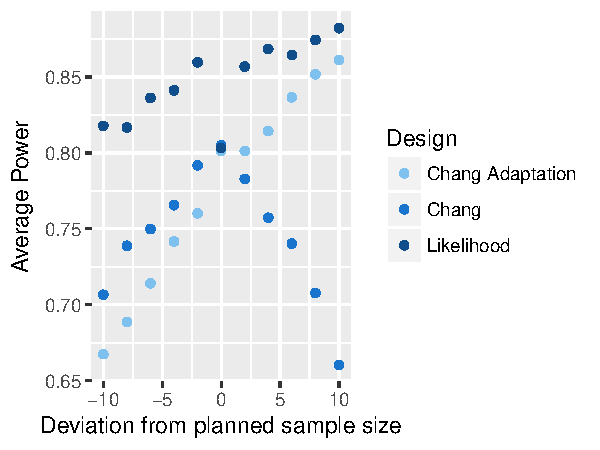
\includegraphics{unnamed-chunk-5-1} }

\end{Schunk}
\end{figure}
\begin{figure}[]
\caption{Monte Carlo Simulation of Average Power of 20 Simon-like Designs when Stage I Sample Size Deviates from Planned for Attained Designs ($n_t^{\ast\ast} = n_1^{\ast\ast} + n_2$) Number of Simulations = 10.}
\centering
\begin{Schunk}


\centerline{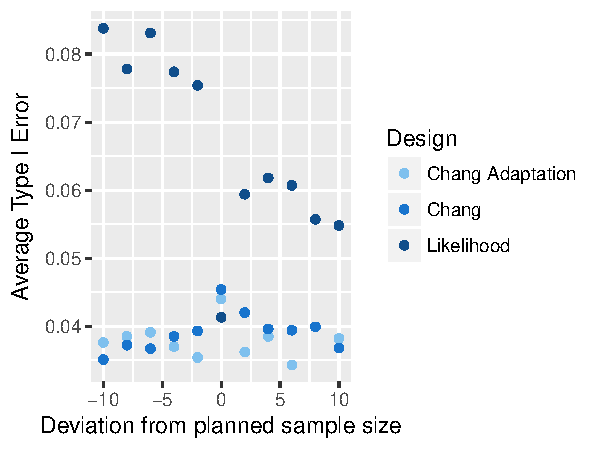
\includegraphics{unnamed-chunk-6-1} }

\end{Schunk}
\end{figure}
\indent We present results that are limited to our primary problem of interest in Tables 6.1 through 6.6. In each design table, the planned design is specified and the first stage sample size varies from planned, while maintaining the original total sample size. We compare attained methods characteristics, in particular, type I error, power, probability of early termination under the null hypothesis, and expected sample size under the null hypothesis. We refer to the Likelihood redesign, Chang and adaptation to Chang redesigns as ``attained methods." \\
\indent Table 6.1 displays a planned Admissible design with varying first stage sample size $\pm$ 10. We notice that under low $p_0$ and $p_1$, $s_1$ will vary between each method. Though, power and type I error are likely to be similar between and within each attained method, and expected sample size is also consistent. The Likelihood and Chang method are at risk of low probability of early termination, especially when the sample size is lower than planned. Table 6.2 shows an Optimal design when $p_0$ is 0.5. Between attained designs, particularly when there is overaccrual, $s_1$ is inconsistent. We particularly see a large difference when $n_1^{\ast\ast} = n_1 + 10$ between the Likelihood and Olson and Koyama designs and the Chang design.  The Likelihood design is anticonservative in type I error and conservative in type II error here, displaying a $\alpha^{\ast\ast} > \alpha$ and $1-\beta^{\ast\ast} > 1-\beta$. The Chang designs both have a conservative type I error for all sample size deviations, though Chang and Likelihood designs maintain higher power than Olson and Koyama's. Probability of early termination is closest to the original under Olson and Koyama's, and thus have a much lower expected sample size under the null hypothesis, with as much as a difference of approximately 23.\\
\indent Table 6.3 displays results from a planned Minimax design when $p_0$ is larger than 0.5. Here, the Likelihood design has desirable properties with type I error and power consistently closed to the planned design for all deviations in sample size. Though, when the sample size is severely underaccrued, the probability of early termination nearly halves. The expected sample size is consistent between designs. The Chang designs stray from the planned nominal type I and type II errors when there is overaccrual. The $\mbox{PET}_0$ for the original Chang design varies significantly between deviations. \\
\indent Table 6.4 through 6.6 display results for planned designs when $\alpha = \beta = 0.1$. Table 6.4 displays attained design characteristics for deviations in sample size when the planned first stage sample size is low. In all three attained designs, we see that as the attained sample size is lower than planned, there is a significant drop in power and a moderate to severe drop in type I error. The probability of early termination almost occurs with probability 1 when the attained sample size is $n_1^{\ast\ast} = 1$. In practice, though, accrual lower than planned here is not practical. When there is overaccrual, attained design characteristics are not concerning. \\
\indent Table 6.5 illustrates the similarity between attained designs when $p_0$ = 0.3. All designs and their deviations are relatively consistent in type I error, power, and $\mbox{PET}_0$. Though, the Olson and Koyama's design is most consistent in the probability of early termination with the planned design, but we see a conservative deviation in type I error for large overaccrual. Table 6.6 displays similar results as Table 5.3. \\




\begin{landscape}

%%%%%%%%%%%%%%%%%%%%%%
%% Table 1
%%%%%%%%%%%%%%%%%%%%%%
\begin{table}[]
\caption{Attained design characteristics from deviation of Admissible II stage design ($p_0$ = 0.1, $p_1$ = 0.25, $\alpha$ = 0.05, $\beta$ = 0.20)}
\small
  \resizebox{\columnwidth}{!}{%

\begin{tabular}{ccccccccccccccccccccccccccc}
  \hline
    \multicolumn{7}{c}{Planned Design}&\multicolumn{3}{r}{Attained Sample Size}&\multicolumn{8}{r}{Redesign}\\
  \multicolumn{8}{c}{     }&\multicolumn{1}{l}{  }&\multicolumn{6}{l}{Chang Design}&\multicolumn{6}{l}{Olson and Koyama Design}&\multicolumn{6}{l}{Likelihood Design}\\
$p_0$ & $p_1$ & $n_1$ & $n$ & $r_1$ & $r_t$ & $\mbox{PET}_0$ &$\mbox{EN}_0$ & $n_1^{\ast\ast}$ & $s_1$ & $s_t$ & $\alpha^{\ast\ast}$ & $1-\beta^{\ast\ast}$ & $\mbox{PET}_0^{\ast\ast}$ & $\mbox{EN}_0^{\ast\ast}$ & $s_1$ & $s_t$ & $\alpha^{\ast\ast}$ & $1-\beta^{\ast\ast}$ & $\mbox{PET}_0^{\ast\ast}$ & $\mbox{EN}_0^{\ast\ast}$ & $s_1$ & $s_t$ & $\alpha^{\ast\ast}$ & $1-\beta^{\ast\ast}$ & $\mbox{PET}_0^{\ast\ast}$ & $\mbox{EN}_0^{\ast\ast}$ \\ 
  \hline
0.1 & 0.25 & 15 & 41 & 1 & 7 & 0.549 & 26.725 & 5 & 0 & 7 & 0.034 & 0.671 & 0.590 & 19.742 & 0 & 7 & 0.034 & 0.671 & 0.590 & 19.742 & 0 & 7 & 0.034 & 0.671 & 0.590 & 19.742 \\ 
  0.1 & 0.25 & 15 & 41 & 1 & 7 & 0.549 & 26.725 & 7 & 0 & 7 & 0.040 & 0.754 & 0.478 & 24.738 & 0 & 7 & 0.040 & 0.754 & 0.478 & 24.738 & 0 & 7 & 0.040 & 0.754 & 0.478 & 24.738 \\ 
  0.1 & 0.25 & 15 & 41 & 1 & 7 & 0.549 & 26.725 & 9 & 0 & 7 & 0.043 & 0.797 & 0.387 & 28.603 & 0 & 7 & 0.043 & 0.797 & 0.387 & 28.603 & 0 & 7 & 0.043 & 0.797 & 0.387 & 28.603 \\ 
  0.1 & 0.25 & 15 & 41 & 1 & 7 & 0.549 & 26.725 & 11 & 0 & 7 & 0.045 & 0.819 & 0.314 & 31.586 & 1 & 7 & 0.035 & 0.718 & 0.697 & 20.079 & 0 & 7 & 0.045 & 0.819 & 0.314 & 31.586 \\ 
  0.1 & 0.25 & 15 & 41 & 1 & 7 & 0.549 & 26.725 & 13 & 0 & 7 & 0.046 & 0.830 & 0.254 & 33.883 & 1 & 7 & 0.040 & 0.771 & 0.621 & 23.602 & 0 & 7 & 0.046 & 0.830 & 0.254 & 33.883 \\ 
  0.1 & 0.25 & 15 & 41 & 1 & 7 & 0.549 & 26.725 & 15 & 1 & 7 & 0.043 & 0.803 & 0.549 & 26.725 & 1 & 7 & 0.043 & 0.803 & 0.549 & 26.725 & 1 & 7 & 0.043 & 0.803 & 0.549 & 26.725 \\ 
  0.1 & 0.25 & 15 & 41 & 1 & 7 & 0.549 & 26.725 & 17 & 1 & 7 & 0.045 & 0.821 & 0.482 & 29.437 & 1 & 7 & 0.045 & 0.821 & 0.482 & 29.437 & 1 & 7 & 0.045 & 0.821 & 0.482 & 29.437 \\ 
  0.1 & 0.25 & 15 & 41 & 1 & 7 & 0.549 & 26.725 & 19 & 2 & 7 & 0.041 & 0.792 & 0.705 & 25.480 & 1 & 7 & 0.046 & 0.831 & 0.420 & 31.754 & 1 & 7 & 0.046 & 0.831 & 0.420 & 31.754 \\ 
  0.1 & 0.25 & 15 & 41 & 1 & 7 & 0.549 & 26.725 & 21 & 2 & 7 & 0.044 & 0.814 & 0.648 & 28.032 & 2 & 7 & 0.044 & 0.814 & 0.648 & 28.032 & 1 & 7 & 0.047 & 0.836 & 0.365 & 33.705 \\ 
  0.1 & 0.25 & 15 & 41 & 1 & 7 & 0.549 & 26.725 & 23 & 3 & 7 & 0.040 & 0.785 & 0.807 & 26.469 & 2 & 7 & 0.046 & 0.827 & 0.592 & 30.345 & 2 & 7 & 0.046 & 0.827 & 0.592 & 30.345 \\ 
  0.1 & 0.25 & 15 & 41 & 1 & 7 & 0.549 & 26.725 & 25 & 3 & 7 & 0.043 & 0.810 & 0.764 & 28.783 & 2 & 7 & 0.047 & 0.834 & 0.537 & 32.406 & 2 & 7 & 0.047 & 0.834 & 0.537 & 32.406 \\ 
   \hline
\end{tabular}
}
\end{table}

%%%%%%%%%%%%%%%%%%%%%%
%% Table 2
%%%%%%%%%%%%%%%%%%%%%%
\begin{table}[]
\caption{Attained design characteristics from deviation of Simon's Optimal II stage design ($p_0$ = 0.5, $p_1$ = 0.65, $\alpha$ = 0.05, $\beta$ = 0.2)}
\small
  \resizebox{\columnwidth}{!}{%

\begin{tabular}{ccccccccccccccccccccccccccc}
  \hline
    \multicolumn{7}{c}{Planned Design}&\multicolumn{3}{r}{Attained Sample Size}&\multicolumn{8}{r}{Redesign}\\
  \multicolumn{8}{c}{     }&\multicolumn{1}{l}{  }&\multicolumn{6}{l}{Chang Design}&\multicolumn{6}{l}{Olson and Koyama Design}&\multicolumn{6}{l}{Likelihood Design}\\
$p_0$ & $p_1$ & $n_1$ & $n$ & $r_1$ & $r_t$ & $\mbox{PET}_0$ &$\mbox{EN}_0$ & $n_1^{\ast\ast}$ & $s_1$ & $s_t$ & $\alpha^{\ast\ast}$ & $1-\beta^{\ast\ast}$ & $\mbox{PET}_0^{\ast\ast}$ & $\mbox{EN}_0^{\ast\ast}$ & $s_1$ & $s_t$ & $\alpha^{\ast\ast}$ & $1-\beta^{\ast\ast}$ & $\mbox{PET}_0^{\ast\ast}$ & $\mbox{EN}_0^{\ast\ast}$ & $s_1$ & $s_t$ & $\alpha^{\ast\ast}$ & $1-\beta^{\ast\ast}$ & $\mbox{PET}_0^{\ast\ast}$ & $\mbox{EN}_0^{\ast\ast}$ \\ 
  \hline
0.5 & 0.65 & 28 & 83 & 15 & 48 & 0.714 & 43.719 & 18 & 8 & 49 & 0.036 & 0.815 & 0.407 & 56.528 & 10 & 48 & 0.037 & 0.685 & 0.760 & 33.622 & 9 & 48 & 0.048 & 0.796 & 0.593 & 44.472 \\ 
  0.5 & 0.65 & 28 & 83 & 15 & 48 & 0.714 & 43.719 & 20 & 10 & 48 & 0.050 & 0.811 & 0.588 & 45.950 & 11 & 48 & 0.039 & 0.716 & 0.748 & 35.859 & 10 & 48 & 0.050 & 0.811 & 0.588 & 45.950 \\ 
  0.5 & 0.65 & 28 & 83 & 15 & 48 & 0.714 & 43.719 & 22 & 11 & 49 & 0.034 & 0.788 & 0.584 & 47.370 & 12 & 48 & 0.042 & 0.743 & 0.738 & 37.966 & 11 & 48 & 0.051 & 0.824 & 0.584 & 47.370 \\ 
  0.5 & 0.65 & 28 & 83 & 15 & 48 & 0.714 & 43.719 & 24 & 12 & 49 & 0.034 & 0.798 & 0.581 & 48.745 & 13 & 48 & 0.044 & 0.765 & 0.729 & 39.967 & 12 & 48 & 0.052 & 0.835 & 0.581 & 48.745 \\ 
  0.5 & 0.65 & 28 & 83 & 15 & 48 & 0.714 & 43.719 & 26 & 14 & 48 & 0.045 & 0.785 & 0.721 & 41.880 & 14 & 48 & 0.045 & 0.785 & 0.721 & 41.880 & 13 & 48 & 0.053 & 0.845 & 0.577 & 50.083 \\ 
  0.5 & 0.65 & 28 & 83 & 15 & 48 & 0.714 & 43.719 & 28 & 15 & 48 & 0.047 & 0.802 & 0.714 & 43.719 & 15 & 48 & 0.047 & 0.802 & 0.714 & 43.719 & 15 & 48 & 0.047 & 0.802 & 0.714 & 43.719 \\ 
  0.5 & 0.65 & 28 & 83 & 15 & 48 & 0.714 & 43.719 & 30 & 16 & 48 & 0.049 & 0.816 & 0.708 & 45.494 & 16 & 48 & 0.049 & 0.816 & 0.708 & 45.494 & 16 & 48 & 0.049 & 0.816 & 0.708 & 45.494 \\ 
  0.5 & 0.65 & 28 & 83 & 15 & 48 & 0.714 & 43.719 & 32 & 17 & 49 & 0.033 & 0.793 & 0.702 & 47.214 & 17 & 49 & 0.033 & 0.793 & 0.702 & 47.214 & 17 & 48 & 0.050 & 0.828 & 0.702 & 47.214 \\ 
  0.5 & 0.65 & 28 & 83 & 15 & 48 & 0.714 & 43.719 & 34 & 19 & 48 & 0.043 & 0.782 & 0.804 & 43.592 & 18 & 49 & 0.034 & 0.803 & 0.696 & 48.886 & 18 & 48 & 0.051 & 0.839 & 0.696 & 48.886 \\ 
  0.5 & 0.65 & 28 & 83 & 15 & 48 & 0.714 & 43.719 & 36 & 20 & 48 & 0.045 & 0.798 & 0.797 & 45.518 & 19 & 49 & 0.035 & 0.811 & 0.691 & 50.516 & 19 & 48 & 0.053 & 0.848 & 0.691 & 50.516 \\ 
  0.5 & 0.65 & 28 & 83 & 15 & 48 & 0.714 & 43.719 & 38 & 21 & 48 & 0.047 & 0.813 & 0.791 & 47.398 & 20 & 49 & 0.035 & 0.818 & 0.686 & 52.110 & 20 & 48 & 0.054 & 0.856 & 0.686 & 52.110 \\
   \hline
\end{tabular}
}
\end{table}

%%%%%%%%%%%%%%%%%%%%%%
%% Table 3
%%%%%%%%%%%%%%%%%%%%%%
\begin{table}[]
\caption{Attained design characteristics from deviation of Simon's Minimax II stage design ($p_0$ = 0.75, $p_1$ = 0.9, $\alpha$ = 0.05, $\beta$ = 0.2)}
\small
  \resizebox{\columnwidth}{!}{%

\begin{tabular}{ccccccccccccccccccccccccccc}
  \hline
    \multicolumn{7}{c}{Planned Design}&\multicolumn{3}{r}{Attained Sample Size}&\multicolumn{8}{r}{Redesign}\\
  \multicolumn{8}{c}{     }&\multicolumn{1}{l}{  }&\multicolumn{6}{l}{Chang Design}&\multicolumn{6}{l}{Olson and Koyama Design}&\multicolumn{6}{l}{Likelihood Design}\\
$p_0$ & $p_1$ & $n_1$ & $n$ & $r_1$ & $r_t$ & $\mbox{PET}_0$ &$\mbox{EN}_0$ & $n_1^{\ast\ast}$ & $s_1$ & $s_t$ & $\alpha^{\ast\ast}$ & $1-\beta^{\ast\ast}$ & $\mbox{PET}_0^{\ast\ast}$ & $\mbox{EN}_0^{\ast\ast}$ & $s_1$ & $s_t$ & $\alpha^{\ast\ast}$ & $1-\beta^{\ast\ast}$ & $\mbox{PET}_0^{\ast\ast}$ & $\mbox{EN}_0^{\ast\ast}$ & $s_1$ & $s_t$ & $\alpha^{\ast\ast}$ & $1-\beta^{\ast\ast}$ & $\mbox{PET}_0^{\ast\ast}$ & $\mbox{EN}_0^{\ast\ast}$ \\ 
  \hline
0.75 & 0.9 & 22 & 39 & 17 & 33 & 0.677 & 27.499 & 12 & 8 & 34 & 0.019 & 0.648 & 0.351 & 29.517 & 9 & 33 & 0.045 & 0.763 & 0.609 & 22.548 & 8 & 33 & 0.050 & 0.805 & 0.351 & 29.517 \\ 
  0.75 & 0.9 & 22 & 39 & 17 & 33 & 0.677 & 27.499 & 14 & 10 & 33 & 0.050 & 0.800 & 0.479 & 27.033 & 11 & 33 & 0.042 & 0.738 & 0.719 & 21.028 & 10 & 33 & 0.050 & 0.800 & 0.479 & 27.033 \\ 
  0.75 & 0.9 & 22 & 39 & 17 & 33 & 0.677 & 27.499 & 16 & 12 & 33 & 0.048 & 0.792 & 0.595 & 25.315 & 12 & 33 & 0.048 & 0.792 & 0.595 & 25.315 & 11 & 33 & 0.051 & 0.809 & 0.370 & 30.494 \\ 
  0.75 & 0.9 & 22 & 39 & 17 & 33 & 0.677 & 27.499 & 18 & 13 & 34 & 0.019 & 0.650 & 0.481 & 28.892 & 14 & 33 & 0.047 & 0.782 & 0.694 & 24.419 & 13 & 33 & 0.051 & 0.807 & 0.481 & 28.892 \\ 
  0.75 & 0.9 & 22 & 39 & 17 & 33 & 0.677 & 27.499 & 20 & 15 & 34 & 0.019 & 0.650 & 0.585 & 27.882 & 15 & 34 & 0.019 & 0.650 & 0.585 & 27.882 & 15 & 33 & 0.050 & 0.805 & 0.585 & 27.882 \\ 
  0.75 & 0.9 & 22 & 39 & 17 & 33 & 0.677 & 27.499 & 22 & 17 & 33 & 0.050 & 0.802 & 0.677 & 27.499 & 17 & 33 & 0.050 & 0.802 & 0.677 & 27.499 & 17 & 33 & 0.050 & 0.802 & 0.677 & 27.499 \\ 
  0.75 & 0.9 & 22 & 39 & 17 & 33 & 0.677 & 27.499 & 24 & 19 & 33 & 0.049 & 0.798 & 0.753 & 27.700 & 19 & 33 & 0.049 & 0.798 & 0.753 & 27.700 & 18 & 33 & 0.051 & 0.810 & 0.578 & 30.332 \\ 
  0.75 & 0.9 & 22 & 39 & 17 & 33 & 0.677 & 27.499 & 26 & 21 & 33 & 0.048 & 0.791 & 0.816 & 28.397 & 20 & 34 & 0.019 & 0.650 & 0.663 & 30.383 & 20 & 33 & 0.051 & 0.810 & 0.663 & 30.383 \\ 
  0.75 & 0.9 & 22 & 39 & 17 & 33 & 0.677 & 27.499 & 28 & 23 & 33 & 0.046 & 0.782 & 0.865 & 29.489 & 22 & 34 & 0.019 & 0.650 & 0.736 & 30.902 & 22 & 33 & 0.051 & 0.810 & 0.736 & 30.902 \\ 
  0.75 & 0.9 & 22 & 39 & 17 & 33 & 0.677 & 27.499 & 30 & 25 & 33 & 0.043 & 0.770 & 0.902 & 30.881 & 23 & 34 & 0.019 & 0.650 & 0.652 & 33.132 & 23 & 33 & 0.051 & 0.810 & 0.652 & 33.132 \\ 
  0.75 & 0.9 & 22 & 39 & 17 & 33 & 0.677 & 27.499 & 32 & 26 & 34 & 0.019 & 0.650 & 0.847 & 33.071 & 25 & 34 & 0.019 & 0.650 & 0.722 & 33.945 & 25 & 33 & 0.051 & 0.810 & 0.722 & 33.945 \\ 
   \hline
\end{tabular}
}
\end{table}

%%%%%%%%%%%%%%%%%%%%%%
%% Table 5
%%%%%%%%%%%%%%%%%%%%%%
\begin{table}[]
\caption{Attained design characteristics from deviation of Simon's Optimal II stage design ($p_0$ = 0.05, $p_1$ = 0.25, $\alpha$ = 0.1, $\beta$ = 0.1)}
\small
  \resizebox{\columnwidth}{!}{%

\begin{tabular}{ccccccccccccccccccccccccccc}
  \hline
    \multicolumn{7}{c}{Planned Design}&\multicolumn{3}{r}{Attained Sample Size}&\multicolumn{8}{r}{Redesign}\\
  \multicolumn{8}{c}{     }&\multicolumn{1}{l}{  }&\multicolumn{6}{l}{Chang Design}&\multicolumn{6}{l}{Olson and Koyama Design}&\multicolumn{6}{l}{Likelihood Design}\\
$p_0$ & $p_1$ & $n_1$ & $n$ & $r_1$ & $r_t$ & $\mbox{PET}_0$ &$\mbox{EN}_0$ & $n_1^{\ast\ast}$ & $s_1$ & $s_t$ & $\alpha^{\ast\ast}$ & $1-\beta^{\ast\ast}$ & $\mbox{PET}_0^{\ast\ast}$ & $\mbox{EN}_0^{\ast\ast}$ & $s_1$ & $s_t$ & $\alpha^{\ast\ast}$ & $1-\beta^{\ast\ast}$ & $\mbox{PET}_0^{\ast\ast}$ & $\mbox{EN}_0^{\ast\ast}$ & $s_1$ & $s_t$ & $\alpha^{\ast\ast}$ & $1-\beta^{\ast\ast}$ & $\mbox{PET}_0^{\ast\ast}$ & $\mbox{EN}_0^{\ast\ast}$ \\ 
  \hline
0.05 & 0.2 & 9 & 24 & 0 & 2 & 0.630 & 14.546 & 1 & 0 & 0 & 0.050 & 0.200 & 0.950 & 2.150 & 0 & 0 & 0.050 & 0.200 & 0.950 & 2.150 & 0 & 2 & 0.016 & 0.192 & 0.950 & 2.150 \\ 
  0.05 & 0.2 & 9 & 24 & 0 & 2 & 0.630 & 14.546 & 3 & 0 & 1 & 0.097 & 0.484 & 0.857 & 5.995 & 0 & 1 & 0.097 & 0.484 & 0.857 & 5.995 & 0 & 2 & 0.043 & 0.465 & 0.857 & 5.995 \\ 
  0.05 & 0.2 & 9 & 24 & 0 & 2 & 0.630 & 14.546 & 5 & 0 & 2 & 0.064 & 0.635 & 0.774 & 9.298 & 0 & 2 & 0.064 & 0.635 & 0.774 & 9.298 & 0 & 2 & 0.064 & 0.635 & 0.774 & 9.298 \\ 
  0.05 & 0.2 & 9 & 24 & 0 & 2 & 0.630 & 14.546 & 7 & 0 & 2 & 0.081 & 0.741 & 0.698 & 12.128 & 0 & 2 & 0.081 & 0.741 & 0.698 & 12.128 & 0 & 2 & 0.081 & 0.741 & 0.698 & 12.128 \\ 
  0.05 & 0.2 & 9 & 24 & 0 & 2 & 0.630 & 14.546 & 9 & 0 & 2 & 0.093 & 0.805 & 0.630 & 14.546 & 0 & 2 & 0.093 & 0.805 & 0.630 & 14.546 & 0 & 2 & 0.093 & 0.805 & 0.630 & 14.546 \\ 
  0.05 & 0.2 & 9 & 24 & 0 & 2 & 0.630 & 14.546 & 11 & 0 & 3 & 0.028 & 0.714 & 0.569 & 16.606 & 0 & 3 & 0.028 & 0.714 & 0.569 & 16.606 & 0 & 2 & 0.102 & 0.843 & 0.569 & 16.606 \\ 
  0.05 & 0.2 & 9 & 24 & 0 & 2 & 0.630 & 14.546 & 13 & 0 & 3 & 0.029 & 0.727 & 0.513 & 18.353 & 0 & 3 & 0.029 & 0.727 & 0.513 & 18.353 & 0 & 2 & 0.108 & 0.864 & 0.513 & 18.353 \\ 
  0.05 & 0.2 & 9 & 24 & 0 & 2 & 0.630 & 14.546 & 15 & 1 & 2 & 0.086 & 0.802 & 0.829 & 16.539 & 0 & 3 & 0.029 & 0.733 & 0.463 & 19.830 & 0 & 2 & 0.112 & 0.876 & 0.463 & 19.830 \\ 
  0.05 & 0.2 & 9 & 24 & 0 & 2 & 0.630 & 14.546 & 17 & 1 & 2 & 0.098 & 0.842 & 0.792 & 18.454 & 1 & 2 & 0.098 & 0.842 & 0.792 & 18.454 & 0 & 2 & 0.114 & 0.882 & 0.418 & 21.073 \\ 
   \hline
\end{tabular}
}
\end{table}


%%%%%%%%%%%%%%%%%%%%%%
%% Table 4
%%%%%%%%%%%%%%%%%%%%%%
\begin{table}[]
\caption{Attained design characteristics from deviation of Admissible II stage design ($p_0$ = 0.3, $p_1$ = 0.45, $\alpha$ = 0.1, $\beta$ = 0.1)}
\small
  \resizebox{\columnwidth}{!}{%

\begin{tabular}{ccccccccccccccccccccccccccc}
  \hline
    \multicolumn{7}{c}{Planned Design}&\multicolumn{3}{r}{Attained Sample Size}&\multicolumn{8}{r}{Redesign}\\
  \multicolumn{8}{c}{     }&\multicolumn{1}{l}{  }&\multicolumn{6}{l}{Chang Design}&\multicolumn{6}{l}{Olson and Koyama Design}&\multicolumn{6}{l}{Likelihood Design}\\
$p_0$ & $p_1$ & $n_1$ & $n$ & $r_1$ & $r_t$ & $\mbox{PET}_0$ &$\mbox{EN}_0$ & $n_1^{\ast\ast}$ & $s_1$ & $s_t$ & $\alpha^{\ast\ast}$ & $1-\beta^{\ast\ast}$ & $\mbox{PET}_0^{\ast\ast}$ & $\mbox{EN}_0^{\ast\ast}$ & $s_1$ & $s_t$ & $\alpha^{\ast\ast}$ & $1-\beta^{\ast\ast}$ & $\mbox{PET}_0^{\ast\ast}$ & $\mbox{EN}_0^{\ast\ast}$ & $s_1$ & $s_t$ & $\alpha^{\ast\ast}$ & $1-\beta^{\ast\ast}$ & $\mbox{PET}_0^{\ast\ast}$ & $\mbox{EN}_0^{\ast\ast}$ \\ 
  \hline
0.3 & 0.45 & 37 & 72 & 11 & 26 & 0.566 & 52.181 & 27 & 7 & 26 & 0.099 & 0.902 & 0.411 & 53.492 & 8 & 26 & 0.090 & 0.871 & 0.577 & 46.020 & 7 & 26 & 0.099 & 0.902 & 0.411 & 53.492 \\ 
  0.3 & 0.45 & 37 & 72 & 11 & 26 & 0.566 & 52.181 & 29 & 8 & 26 & 0.097 & 0.897 & 0.479 & 51.416 & 9 & 26 & 0.087 & 0.862 & 0.636 & 44.652 & 8 & 26 & 0.097 & 0.897 & 0.479 & 51.416 \\ 
  0.3 & 0.45 & 37 & 72 & 11 & 26 & 0.566 & 52.181 & 31 & 8 & 27 & 0.065 & 0.870 & 0.386 & 56.155 & 9 & 26 & 0.095 & 0.892 & 0.542 & 49.794 & 8 & 26 & 0.101 & 0.910 & 0.386 & 56.155 \\ 
  0.3 & 0.45 & 37 & 72 & 11 & 26 & 0.566 & 52.181 & 33 & 9 & 26 & 0.100 & 0.907 & 0.450 & 54.460 & 10 & 26 & 0.093 & 0.886 & 0.599 & 48.626 & 9 & 26 & 0.100 & 0.907 & 0.450 & 54.460 \\ 
  0.3 & 0.45 & 37 & 72 & 11 & 26 & 0.566 & 52.181 & 35 & 10 & 26 & 0.099 & 0.904 & 0.510 & 53.132 & 10 & 26 & 0.099 & 0.904 & 0.510 & 53.132 & 10 & 26 & 0.099 & 0.904 & 0.510 & 53.132 \\ 
  0.3 & 0.45 & 37 & 72 & 11 & 26 & 0.566 & 52.181 & 37 & 11 & 26 & 0.097 & 0.901 & 0.566 & 52.181 & 11 & 26 & 0.097 & 0.901 & 0.566 & 52.181 & 11 & 26 & 0.097 & 0.901 & 0.566 & 52.181 \\ 
  0.3 & 0.45 & 37 & 72 & 11 & 26 & 0.566 & 52.181 & 39 & 12 & 26 & 0.095 & 0.897 & 0.618 & 51.601 & 12 & 26 & 0.095 & 0.897 & 0.618 & 51.601 & 11 & 26 & 0.101 & 0.912 & 0.482 & 56.108 \\ 
  0.3 & 0.45 & 37 & 72 & 11 & 26 & 0.566 & 52.181 & 41 & 13 & 26 & 0.094 & 0.893 & 0.665 & 51.372 & 12 & 27 & 0.065 & 0.871 & 0.536 & 55.378 & 12 & 26 & 0.100 & 0.910 & 0.536 & 55.378 \\ 
  0.3 & 0.45 & 37 & 72 & 11 & 26 & 0.566 & 52.181 & 43 & 14 & 26 & 0.091 & 0.889 & 0.708 & 51.466 & 13 & 26 & 0.099 & 0.908 & 0.587 & 54.967 & 13 & 26 & 0.099 & 0.908 & 0.587 & 54.967 \\ 
  0.3 & 0.45 & 37 & 72 & 11 & 26 & 0.566 & 52.181 & 45 & 14 & 26 & 0.098 & 0.906 & 0.635 & 54.864 & 13 & 27 & 0.066 & 0.875 & 0.509 & 58.264 & 13 & 26 & 0.103 & 0.915 & 0.509 & 58.264 \\ 
  0.3 & 0.45 & 37 & 72 & 11 & 26 & 0.566 & 52.181 & 47 & 15 & 26 & 0.097 & 0.904 & 0.678 & 55.050 & 14 & 27 & 0.066 & 0.874 & 0.559 & 58.028 & 14 & 26 & 0.102 & 0.914 & 0.559 & 58.028 \\  
   \hline
\end{tabular}
}
\end{table}











%%%%%%%%%%%%%%%%%%%%%%
%% Table 6
%%%%%%%%%%%%%%%%%%%%%%
\begin{table}[]
\caption{Attained design characteristics from deviation of Simon's Minimax II stage design ($p_0$ = 0.75, $p_1$ = 0.9, $\alpha$ = 0.1, $\beta$ = 0.1)}
\small
  \resizebox{\columnwidth}{!}{%

\begin{tabular}{ccccccccccccccccccccccccccc}
  \hline
    \multicolumn{7}{c}{Planned Design}&\multicolumn{3}{r}{Attained Sample Size}&\multicolumn{8}{r}{Redesign}\\
  \multicolumn{8}{c}{     }&\multicolumn{1}{l}{  }&\multicolumn{6}{l}{Chang Design}&\multicolumn{6}{l}{Olson and Koyama Design}&\multicolumn{6}{l}{Likelihood Design}\\
$p_0$ & $p_1$ & $n_1$ & $n$ & $r_1$ & $r_t$ & $\mbox{PET}_0$ &$\mbox{EN}_0$ & $n_1^{\ast\ast}$ & $s_1$ & $s_t$ & $\alpha^{\ast\ast}$ & $1-\beta^{\ast\ast}$ & $\mbox{PET}_0^{\ast\ast}$ & $\mbox{EN}_0^{\ast\ast}$ & $s_1$ & $s_t$ & $\alpha^{\ast\ast}$ & $1-\beta^{\ast\ast}$ & $\mbox{PET}_0^{\ast\ast}$ & $\mbox{EN}_0^{\ast\ast}$ & $s_1$ & $s_t$ & $\alpha^{\ast\ast}$ & $1-\beta^{\ast\ast}$ & $\mbox{PET}_0^{\ast\ast}$ & $\mbox{EN}_0^{\ast\ast}$ \\ 
  \hline
0.75 & 0.9 & 27 & 40 & 20 & 33 & 0.529 & 33.121 & 17 & 11 & 33 & 0.096 & 0.900 & 0.235 & 34.602 & 12 & 33 & 0.094 & 0.895 & 0.426 & 30.199 & 11 & 33 & 0.096 & 0.900 & 0.235 & 34.602 \\ 
  0.75 & 0.9 & 27 & 40 & 20 & 33 & 0.529 & 33.121 & 19 & 13 & 33 & 0.096 & 0.900 & 0.332 & 33.023 & 14 & 33 & 0.092 & 0.890 & 0.535 & 28.774 & 13 & 33 & 0.096 & 0.900 & 0.332 & 33.023 \\ 
  0.75 & 0.9 & 27 & 40 & 20 & 33 & 0.529 & 33.121 & 21 & 15 & 33 & 0.095 & 0.899 & 0.433 & 31.765 & 15 & 33 & 0.095 & 0.899 & 0.433 & 31.765 & 14 & 33 & 0.096 & 0.900 & 0.256 & 35.129 \\ 
  0.75 & 0.9 & 27 & 40 & 20 & 33 & 0.529 & 33.121 & 23 & 16 & 33 & 0.096 & 0.900 & 0.346 & 34.113 & 17 & 33 & 0.095 & 0.898 & 0.532 & 30.964 & 16 & 33 & 0.096 & 0.900 & 0.346 & 34.113 \\ 
  0.75 & 0.9 & 27 & 40 & 20 & 33 & 0.529 & 33.121 & 25 & 18 & 33 & 0.096 & 0.900 & 0.439 & 33.416 & 18 & 33 & 0.096 & 0.900 & 0.439 & 33.416 & 18 & 33 & 0.096 & 0.900 & 0.439 & 33.416 \\ 
  0.75 & 0.9 & 27 & 40 & 20 & 33 & 0.529 & 33.121 & 27 & 20 & 33 & 0.096 & 0.900 & 0.529 & 33.121 & 20 & 33 & 0.096 & 0.900 & 0.529 & 33.121 & 20 & 33 & 0.096 & 0.900 & 0.529 & 33.121 \\ 
  0.75 & 0.9 & 27 & 40 & 20 & 33 & 0.529 & 33.121 & 29 & 22 & 33 & 0.096 & 0.900 & 0.613 & 33.255 & 22 & 33 & 0.096 & 0.900 & 0.613 & 33.255 & 21 & 33 & 0.096 & 0.900 & 0.443 & 35.124 \\ 
  0.75 & 0.9 & 27 & 40 & 20 & 33 & 0.529 & 33.121 & 31 & 24 & 33 & 0.096 & 0.900 & 0.688 & 33.805 & 23 & 33 & 0.096 & 0.900 & 0.527 & 35.255 & 23 & 33 & 0.096 & 0.900 & 0.527 & 35.255 \\ 
  0.75 & 0.9 & 27 & 40 & 20 & 33 & 0.529 & 33.121 & 33 & 26 & 33 & 0.096 & 0.900 & 0.753 & 34.727 & 25 & 33 & 0.096 & 0.900 & 0.606 & 35.757 & 25 & 33 & 0.096 & 0.900 & 0.606 & 35.757 \\ 
  0.75 & 0.9 & 27 & 40 & 20 & 33 & 0.529 & 33.121 & 35 & 28 & 33 & 0.096 & 0.900 & 0.808 & 35.960 & 26 & 33 & 0.096 & 0.900 & 0.526 & 37.372 & 26 & 33 & 0.096 & 0.900 & 0.526 & 37.372 \\ 
  0.75 & 0.9 & 27 & 40 & 20 & 33 & 0.529 & 33.121 & 37 & 30 & 33 & 0.096 & 0.900 & 0.853 & 37.441 & 28 & 33 & 0.096 & 0.900 & 0.600 & 38.199 & 28 & 33 & 0.096 & 0.900 & 0.600 & 38.199 \\ 
   \hline
\end{tabular}
}
\end{table}



\end{landscape}

\indent Figures 6.3 and 6.4 display Monte Carlo simulation results for type I error and power, respectively. The results are an average of 20 Simon-like designs with $\alpha = 0.05, \beta = 0.2$ and stage I sample size deviations with $n_t^{\ast\ast} = n_t$ for each attained design method. Therefore, each point will be an average of attained type I error or power under different sample size deviations. We see that, on average, the Likelihood two-stage design has power above the nominal power and below the nominal alpha level for all sample size deviations $\pm 10$. Both Chang's and Olson and Koyama's methods are conservative in type I error for all sample size deviations, but are more likely to suffer in power. Figure 6.5 shows a similar Monte Carlo simulation, though it displays the average of the average type I error rate and the average type II error rate. The simulation confirms that the Likelihood design minimizes the average of the error rates, while Chang \textit{et al.}'s method performs better in this sense when there is under-enrollment, while Olson and Koyama performs better when there is over-enrollment.\\


\begin{figure}[]
\caption{Monte Carlo Simulation of Average Power of 20 Simon-like Designs when Stage I Sample Size Deviates from Planned for Attained Designs ($n_t^{\ast\ast} = n_t$) Number of Simulations = 10.}
\begin{Schunk}


\centerline{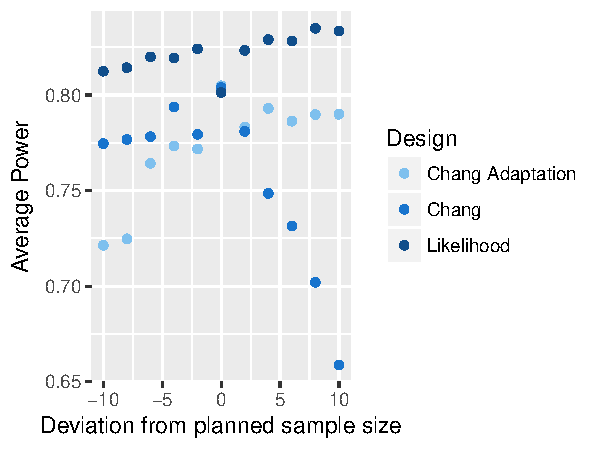
\includegraphics{unnamed-chunk-14-1} }

\end{Schunk}
\end{figure}

\begin{figure}[]
\caption{Monte Carlo Simulation of Average Type I Error Rates of 20 Simon-like Designs when Stage I Sample Size Deviates from Planned for Attained Designs ($n_t^{\ast\ast} = n_t$) Number of Simulations = 10.}
\begin{Schunk}


\centerline{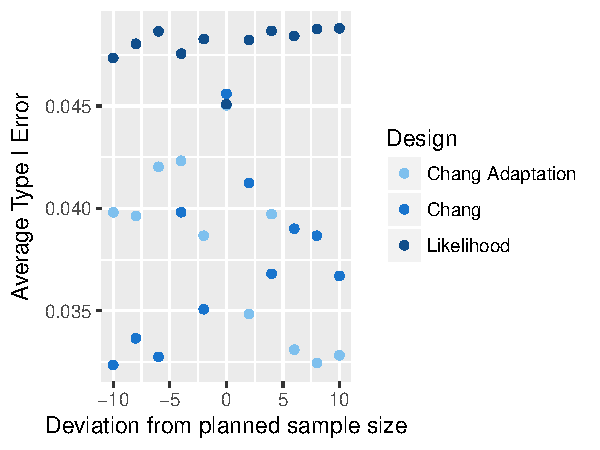
\includegraphics{unnamed-chunk-15-1} }

\end{Schunk}
\end{figure}

\begin{figure}[]
\caption{Monte Carlo Simulation of the Average of the Average Type I and Type II Error Rates of 20 Simon-like Designs when Stage I Sample Size Deviates from Planned for Attained Designs ($n_t^{\ast\ast} = n_t$) Number of Simulations = 10.}
\begin{Schunk}


\centerline{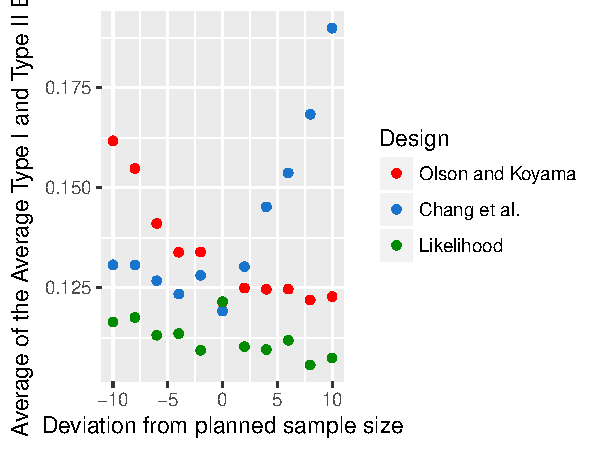
\includegraphics{unnamed-chunk-16-1} }

\end{Schunk}
\end{figure}

%%%%%%%%%%%%%%%%%%%%%%%%%%%%%%%%%%%%%%%%%%%%%%%%%%%%%%%%%%%%%%
%----------------Discussion--------------------------------%
\newpage
\chapter{Discussion and Conclusion}

%%%%%%%%%%%%%%%%%%%%%%%%%%%%%%%%%%%%%%%%%%%%%%%%%%%%%%%%%%%%%%
Deviations from the planned second stage sample size has been better studied than deviations from the planned first stage sample size. Many methods have been proposed on decision rules, and Koyama \textit{et al}. had introduced a redesign when the first stage sample size is as planned. Because the calculation of a p-value in this case is more straightforward than when stage I differs, there may be less literature proposing redesigns. One could calculate a p-value ignoring the sample paths for deviations in either the first or second stage, though, as if the two-stage design was a single stage with attained values. If this was done, the decision could be different than the p-value considering sample paths and how to decide how small the p-value is needed in order to determine statistical significance is unclear. Here, we focused our investigation and results on deviations from the planned first stage sample size. One argument against redesigning these trials in the first place could be that researchers always have the option to simply wait until stage I sample size is met. In practice, though, some ethical matters may arise that would give the researcher incentive to evaluate the first stage prematurely. For instance, if a new regimen appears to be more beneficial than historical treatments, but statistical requirements prevent new subjects from being enrolled until all currently enrolled subjects record responses, a researcher may consider this unethical. In this case, $n_1^{\ast\ast} < n_1$ where $n_1^{\ast\ast}$ would be subjects who have recorded responses. Having a decision rule for a case such as this would alleviate some discomfort from both the researcher and statistician, though abuse of new decision rules would be discouraged. \\
\indent A numerical study suggested that it may be desirable to redesign trials using the planned total sample size because it better controls type I error for all attained methods and power is closer to the nominal power, on average. Assuming that redesigns use the planned total sample size in the redesign, results from different Simon-like designs were presented.  Chang and the Olson and Koyama methods primarily differ when there are extreme sample size shifts. This is most likely due to the nature of their methods and their primary goals of maintaining type II error spending or probability of early termination. \\
\indent Recommending the use of these designs in practice will depend on the desire of statistical approach of the researcher. Blume states, "Hypothesis testing procedures do not place any interpretation on the numerical value of the likelihood ratio. the extremeness of an observation is measured, not by the magnitude of the likelihood ratio, but by the probability of observing a likelihood ratio that large or larger. It is the tail area, not the likelihood ratio, that is the meaningful quantity in hypothesis testing" \cite{Blume2002}. Thus, the primary argument for using Chang \textit{et al.}'s or the OK method is in the case that the researcher does not want to abandon hypothesis testing.  If the researcher prefers to use a traditional Frequentist approach with hypothesis testing, it may be recommended that the Olson and Koyama's approach is used because it results in higher average power across deviations. Because it may be of concern that researchers take advantage of the ability to deviate from the planned design, Olson and Koyama's method also penalizes deviation by resulting in a higher probability of early termination when there is underaccrual than Chang \textit{et al}'s method. \\
\indent Overall, there are many advantages to using a Likelihood two-stage design. One advantage to the Likelihood design is that it is able to add cohorts of subjects at the end of the second stage if weak evidence is obtained without threatening frequentist properties such as type I error. Another advantage to the Likelihood approach is that inference is more straightforward because one is not concerned with error rates or p-values. The likelihood is unaffected by the number of looks at the data and the evidence is independent of the probability of observing misleading evidence \cite{Blume2002}. Though we don't consider calculating p-values when stage I differs from planned, it would be complicated if one wished to do so, whereas Likelihood methods would not require this because evidence is represented by a simple calculation of the likelihood ratio.  Likelihood designs are also more generalizable. The Likelihood two-stage approach could be generalized easily to three stages, whereas the Chang \textit{et al.} and OK designs would not be able to generalize in such a way. In this paper, though, we are very much restricting the Likelihood design and not taking full advantage of its natural characteristics. One could simply use a pure Likelihood design and avoid traditional Frequentist issues altogether. \\
\indent In general, though, if a researcher wanted to design a study using the restricted designs as described in this paper, the OK design and the Likelihood design are highly competitive and achieve similar results when the probability of early termination is reasonable (i.e. above 50\%). One design may be more favorable than the other depending on the hypotheses being tested and the amount of over- or under-enrollment. 
\indent We do not consider redesigns when both the first and second stage accrual are not as planned because if one is interested in prespecifying stopping criteria for sample size deviations, the number of combinations needed to be specified in order to prespecify the exact combination that will occur is unreasonable. Though, these attained designs are able to accommodate if this is desired. Lastly, a primary concern that we have with redesigning trials for unplanned sample sizes is that researchers could take advantage of the these new stopping criteria and stray from the planned design too often. It is for this reason that one may consider adapting Chang \textit{et al.}'s design using a very conservative rule in the first stage and have the probability of early termination under the null always be higher than planned. When deviations are extreme, especially where there is underacrrual, evaluating the trial early would be highly penalized by potentially having a very high probability of early termination. Overall, intentional early or late evaluation of the first stage without sound reason is highly discouraged and will not result in optimal statistical properties. 




%%%%%%%%%%%%%%%%%%%%%%%%%%%%%%%%%%%%%%%%%%%%%%%%%%%%%%%%%%%%%%
%------------------------------------------------%
%%%%%%%%%%%%%%%%%%%%%%%%%%%%%%%%%%%%%%%%%%%%%%%%%%%%%%%%%%%%%%

%%%%%%%%%%%%%%%%%%%%%%%%%%%%%%%%%%%%%%%%%%%%%%%%%%%%%%%%%%%%%%
%-------------- BIBLIOGRAPHY--------------------------------------%
%%%%%%%%%%%%%%%%%%%%%%%%%%%%%%%%%%%%%%%%%%%%%%%%%%%%%%%%%%%%%%


%\bibliographystyle{apacite}
\bibliographystyle{ieeetr}
\bibliography{/Users/mollyolson/Documents/Vanderbilt/Masters_Thesis/ThesisRepo/thesisBib}		

\end{document} 


